%%===================================
\documentclass[12pt, a4paper, twoside, norsk, openright, notitlepage]{report}
\usepackage{settings/main}
\newacronym{iot}{IoT}{tingenes internett}
\newacronym{aws}{AWS}{Amazon Web Services}
\newacronym{mqtt}{MQTT}{\textit{MQ Telemetry Transport}}
\newacronym{copd}{COPD}{Chronic Obstructive Pulmonary Disease}
\newacronym{api}{API}{\textit{Application Programming Interface}}
\newacronym{tcp}{TCP}{\textit{Transmission Control Protocol}}
\newacronym{http}{HTTP}{\textit{Hypertext Transfer Protocol}}
\newacronym{iaas}{IaaS}{Infrastructure as a Service}
\newacronym{paas}{PaaS}{Platform as a Service}
\newacronym{ddos}{DDoS}{Distributed Denial of Service}
\newacronym{tls}{TLS}{\textit{Transport Layer Security}}
\newacronym{uri}{URI}{Uniform Resource Identifier}
\newacronym{m2m}{M2M}{Machine to Machine}
\newacronym{amqp}{AMQP}{Advanced Message Queuing Protocol}
\newacronym{ble}{BLE}{\textit{Bluetooth Low Energy}}
\newacronym{npm}{NPM}{«Node Package Manager»}
\newacronym{uuid}{UUID}{Universally unique identifier}
\newacronym{gatt}{GATT}{\textit{Generic Attribute Profile}}
\newacronym{mitm}{MITM}{\textit{man-in-the-middle-angrep}}
\newacronym{gpio}{GPIO}{\textit{general-purpose input/output}}

%%===================================
\begin{document}
\setcounter{page}{0}
\pagenumbering{roman}

\addcontentsline{toc}{chapter}{\abstractname}

\begin{abstract}
\noindent
Kroniske sykdommer er den mest vanlige dødsårsaken på verdensbasis.
Ved å følge opp pasienter i sitt eget hjem med egenrapportering av dagsform
og innrapportering av sensordata, ønsker man å redusere sykehusinnleggelser
og øke trygghet- og mestringsfølelsen. Avstandsoppfølging av kronisk syke
(avstandsoppfølging) er et satsingsområde for
Norge som har bevilget 30 millioner til et prosjekt for å teste ut dette i fire
kommuner: Sarpsborg, Oslo, Stavanger og Trondheim.

\noindent \newline
I denne masteroppgaven ble en frittstående prototype av et skytilkoblet pulsoksymeter
evaluert for bruk i avstandsoppfølging. Løsningen var basert på en Raspberry Pi
Zero W, en fingeravtrykksensor for autentisering av pasienten, en knapp og tre lysdioder.
Hensiktet med dette var å finne en arkitektur for avstandsoppfølging basert på moderne
tingenes internett (IoT)-skyløsninger lansert i løpet av de siste par årene, og
finne ut hva som vil bli viktige aspekter ved utviklingen av et en slik teknologisk plattform
fremover.

\noindent \newline
Det ble gjennomført en case-studie for å se hvordan Trondheim kommune jobber med
avstandsoppfølging, og hva som er status på det prosjektet i første halvdel av 2017.
To runder med intervjuer av en prosjektleder og en som jobber med velferdsteknologi
i Trondheim kommune ble gjennomført:
først et rent bakgrunnsintervju og deretter et evaluerings- og oppsummeringsintervju
hvor de fikk se på og prøve ut prototypen. Det ble også gjort et evaluerings- og
oppsummeringsintervju med to forskere fra SINTEF.

\noindent \newline
Resultatene viste at en mulig arkitektur for avstandsoppfølging kan realiseres
med skyplattformen AWS IoT som gir god innebygd sikkerhet. Problemet med denne
plattformen er at dataen ikke lagres i Norge, som som har vært et ønske
i Norge for helseapplikasjoner.
Et annet viktig teknisk aspekt som ble avdekket, var at sensorer tidlig
må ta i bruk nye Bluetooth-versjoner -- og helst versjon 4.2 eller nyere.
Den nye personsvernforordningen til EU som implementeres i norsk lov i starten
av 2018 gir brukerne enda mer kontroll over egne data, og kommer
til å få konsekvenser for utviklingen av skybaserte IoT-løsninger i velferdsteknologi.
Trondheim kommune var veldig klar over den juridiske problematikken, og ville jobbe
videre med dette.

\noindent \newline
Trondheim kommune påpekte at det vanskelige med avstandsoppfølging ikke nødvendigvis
er teknologien, men å få løsningen til å fungere i storskala i en kommune med flere
hundre brukere.
De mente at prototypen var enkelt å bruke og kunne vært brukt av
pasienter. De ville kanskje heller ha en løsning med flere sensorer rundt en sentral hub
(som godt kunne være frittstående), enn å ha alt integrert i sensoren. De
så for seg en fremtid der brukeren selv kan velge hva slags løsning de vil bruke
og at kommunen kan være til stede på de plattformene brukeren er fra før av -- det
seg være iOS, Android, PC eller en frittstående løsning.

\noindent \newline
Forskere ved SINTEF mente at
å rapportere dagsform burde vært med i prototypen. Fingeravtrykksensor ville heller
ikke vært en god løsning for alle typer brukere.
De var teknologioptimisiske når
det gjaldt innrapportering av sensordata, og så på automatisk analyse av data
og bedre toveiskommunikasjon som noe positivt å jobbe med videre. Brukerne må få
tilbakemelding og oversikt over målingene sine.
\end{abstract}

\cleardoublepage

\addcontentsline{toc}{chapter}{Abstract}

\begin{otherlanguage}{english} 
\begin{abstract}
Chronic diseases are the most common cause of death worldwide. By following up
on patients in their own homes by self-reporting their daily form and reporting
sensor data, the goals are to reduce hospitalizations and increase the sense of
security and achievement. Remote monitoring of patients with chronic
diseases (remote monitoring) is a priority area for
Norway, which has allocated 30 million NOK to a project to test this in
four municipalities: Sarpsborg, Oslo, Stavanger and Trondheim.

In this master's thesis, a prototype of a stand-alone and cloud-connected
pulse oximeter was evaluated for use in remote monitoring.
The solution was based on a Raspberry Pi Zero W, a fingerprint sensor for
authentication of the patient, one button and three LEDs. The purpose
of this was to find an architecture for remote monitoring based on modern
Internet of Things (IoT) solutions in the cloud released during the last
couple of years, and what the important aspects will be with the development of
such a technological platform in the future.

A case study was conducted to see how the municipality of Trondheim is working
with remote monitoring, and what the current situation is in that project in the
beginning of 2017. To rounds of interviews with a project manager and a person
who works with welfare technology in the municipality of Trondheim were
conducted: first a background interview and then an evaluation and
summary interview where they looked at and tested the prototype. An evaluation
and summary interview with two researchers from SINTEF was also conducted.

The results showed that a possible architecture for remote monitoring can be
realized with the cloud platform AWS IoT, which gives good built-in safety.
The problem with this platform is that the data is not stored in Norway which
has usually been the norm in Norway for health applications.
An other important technical finding, was that sensors must use new versions
of Bluetooth as early as possible, and preferably version 4.2 or later.
The new General Data Protection Regulation (GDPR) from the European Union which
will be implemented in Norway in the beginning of 2018, will give users more
control of their own data, and will have consequences for the development of
cloud IoT solutions in welfare technology. The municipality of Trondheim were
aware of the problems from a legal point of view, and said that they would
continue to work with this.

The municipality of Trondheim pointed out that the difficulty in remote
monitoring is not necessarily the technology, but making the solution work in
large scale in a municipality with hundreds of users. They thought the prototype
was easy to use and could be used by patients. They would perhaps rather have a
solution with sensors around a central hub (which could have been stand-alone)
than having everything be integrated in the sensor. They projected a future
where the user can choose the solution they want to use and that the
municipality can be present on the platforms the users already are on -- for
instance iOS, Android, PC or a stand-alone solution.

The researchers from SINTEF thought that self-reporting the daily form should
have been in the prototype. Also, a fingerprint sensor would not be a good
solution for all types of users. They were optimistic about the technology when
it came to reporting of sensor data, and they viewed automatic analysis of data and
better two-way communication as something positive to work on in the
future. The users must have an overview and get feedback on the measurements
with sensors.
\end{abstract}
\end{otherlanguage}

\cleardoublepage

\phantomsection
\addcontentsline{toc}{chapter}{\prefacename}
\chapter*{Forord}
Takk til veileder professor Dag Svanæs for kjempegod hjelp og tilbakemeldinger gjennom hele prosjektet.

Takk til Terje Røsand ved instituttet for hyggelige samtaler og uvurderlig hjelp med 3D-printing, lodding og elektronikk.
IDI er heldige som har en så stor ressurs som deg.

En stor takk rettes til Trondheim kommune for godt samarbeid og utlån av pulsoksimeter.
Ingar og Renate -- til tross for en veldig travel periode satte dere av tid til meg, takk for det!
Takk til SINTEF for hjelpen med å komme i gang med prosjektet, og for at dere
stilte på evaluering- og oppsummeringsintervju.

\begin{flushright}
Andreas Drivenes\\[0.8pc]
Trondheim, \today
\end{flushright}

\cleardoublepage

\phantomsection
\addcontentsline{toc}{chapter}{\contentsname}
\tableofcontents
\cleardoublepage

\phantomsection
\addcontentsline{toc}{chapter}{\listtablename}
\listoftables
\cleardoublepage

\phantomsection
\addcontentsline{toc}{chapter}{\listfigurename}
\listoffigures									
\cleardoublepage

\phantomsection
\printnoidxglossary[type=\acronymtype,title=Forkortelser]
\cleardoublepage


\makeatletter
\newenvironment{chapquote}[2][2em]
  {\setlength{\@tempdima}{#1}%
   \def\chapquote@author{#2}%
   \parshape 1 \@tempdima \dimexpr\textwidth-2\@tempdima\relax%
   \itshape}
  {\par\normalfont\hfill\ \chapquote@author\hspace*{\@tempdima}\par\bigskip}
\makeatother

\hspace{0pt}
\vfill

\begin{chapquote}{Donald Knuth, \textit{Literate Programming}}
Let us change our traditional attitude to the construction of programs: Instead of imagining that our main task is to instruct a computer what to do, 
let us concentrate rather on explaining to human beings what we want a computer to do.
\end{chapquote}

\vfill
\hspace{0pt}

\iffalse
\vspace*{\fill} 
\def\signed#1{{\unskip\nobreak\hfil\penalty50
    \hskip2em\hbox{}\nobreak\hfil\sl#1
    \parfillskip=0pt \finalhyphendemerits=0 \par}}

\begin{quote} 
Let us change our traditional attitude to the construction of programs: Instead of imagining that our main task is to instruct a computer what to do, 
let us concentrate rather on explaining to human beings what we want a computer to do.

\signed{Donald Knuth}
\end{quote}
\vspace*{\fill}
\fi

\thispagestyle{plain}

\thispagestyle{plain}
\cleardoublepage

%%=========================================
\setcounter{page}{0}
\pagenumbering{arabic}

\chapter{Introduksjon}
\label{ch:introduction}
Hensikten med dette forskningsprosjektet er å evaluere ny teknologi for avstandsoppfølging av kronisk
syke i form av en første prototype av et skytilkoblet pulsoksimeter. Prototypen
vil vises fram for prosjektledere og forskere innen velferdsteknologi for
å avdekke hva som vil bli viktige aspekter ved utviklingen av helseprodukter
basert på \gls{iot}-skyløsninger i fremtiden.
Det overordnete forskningsspørsmålet er: «Hvor egnet er skybasert \acrfull{iot} som teknologisk plattform for avstandsoppfølging av kronisk syke?»
Velferdsteknologiprogrammet i Trondheim kommune og SINTEF bistår prosjektet.

Dette kapittelet beskriver bakgrunnen for forskningsprosjektet: hva som motiverer det,
forskningsspørsmålene som skal besvares og forskingsdesignet som understøtter det,
hvilke begrensninger og avveininger som er gjort og til slutt en disposisjon av oppgaven.

\section{Bakgrunn og motivasjon}
\textquote[\cite{itu_iot}]{\Acrfull{iot} er en global infrastruktur for informasjonssamfunnet som muliggjør avanserte tjenester ved å
knytte sammen fysiske og virtuelle ting basert på eksisterende og fremadstormende kompatible informasjon- og kommunikasjonsteknologier}{.}
\gls{iot} gir nye og spennende muligheter for kreative løsninger på problemer på forskjellige områder, alt fra husholdningsapparater
og fjernoppdatering av programvare i biler, til oppfølging av helseproblemer innen velferdsteknologi. Datakraft- og lagring
har blitt mye billigere, noe som gjør at man i større grad enn tidligere kan samle inn informasjon om verden rundt oss
med sensorer. De to største leverandørene av skytjenester, \gls{aws} og Microsoft Azure,
har i løpet av det siste halvannet året lansert nye tjenester for å få sensorenheter tilkoblet til Internett
på en enkel og sikker måte.

Velferdsteknologi har vært høyt prioritert av helsemyndighetene i Norge de siste årene. Trondheim kommune prøver ut
et prosjekt med avstandsoppfølging av kronisk syke kalt HelsaMi+ på oppdrag fra Helsedirektoratet. 
Avstandsoppfølging kan øke trygghetsfølelsen for innbyggerne og føre til lavere kostnader og færre sykehusinnleggelser (kilde?).
Løsningen til Trondheim kommune innebærer bruk av et nettbrett der man daglig svarer på spørsmål om hvordan formen er. Noen av pasientene
kan måle vekt, blodtrykk, pulsfrekvens og oksygenmetning ved hjelp av sensorer koblet til nettbrettet.

Motivasjonen for dette forskningsprosjektet er å ta i bruk den nye skyteknologien fra \gls{aws} i en frittstående
pulsoksimeterprototype for avstandsoppfølging av kronisk syke som et alternativ til den løsningen Trondheim
kommune tester ut i dag. Det vil gjøre at dette prosjektet kan sammenligne de to løsningene og undersøke hvordan ny
teknologi kan brukes i avstandsoppfølging av kronisk syke. Et pulsoksimeter er en sensor som kan måle pulsfrekvens og oksygenmetning i blodet. 

\section{Forskningsspørsmål}
\label{sec:res_questions}
% @Todo: Noe som presenterer forskningsspørsmålene her?

\begin{enumerate}
  \item[\textbf{FS1}] Hvordan gjøres avstandsoppfølging av kronisk syke i Trondheim dag,
     og hvilke planer finnes for ny teknologi på dette området?
  \item[\textbf{FS2}] Hva er en mulig teknologistakk for realisering av skybasert \gls{iot} for avstandsoppfølging av kronisk syke?
  \item[\textbf{FS3}] Hvordan vurderer domeneeksperter innen velferdsteknologi frittstående skybaserte \gls{iot}-løsninger for avstandsoppfølging av kronisk syke?
  \item[\textbf{FS4}] Basert på funnene fra FS1, FS2 og FS3, hva er implikasjonene for utviklingen av skybasert \gls{iot} som teknologisk plattform
    for avstandsoppfølging av kronisk syke?
\end{enumerate}

Heretter vil «avstandsoppfølging av kronisk syke» bli betegnet som «avstandsoppfølging».

\section{Forskningsmetoder og forskningsdesign}
Rammeverket for å beskrive forskningsprosjektet er hentet fra \citet{oates}. Hovedstrategien for å besvare på \textbf{FS1} i
delkapittel \ref{sec:res_questions} er å gjøre en liten case-studie på hvordan avstandsoppfølging foregår i Trondheim kommune. Datagenereringsmetoder
er intervjuer og dokumenter. 

For å svare på \textbf{FS2} og \textbf{FS3} vil den primære strategien være \textit{design og kreasjon} (prototyping/\textit{proof of concept})
med intervjuer og dokumenter som datageneringsmetode. Case-studien vil også hjelpe til med å besvare disse spørsmålene. \textbf{FS4} vil drøftes kvalitativt 
utifra svarene på de andre forskningsspørsmålene. Det vil kun gjøres kvalitative dataanalyser.

Forskningsmetodene og forskningsdesignet er utdypet i kapittel \ref{ch:method} og \ref{ch:design}.

\section{Avgrensning av forskningen}
Om man kan gjøre kliniske vurderinger basert på sensordataene, kommer ikke til å være i søkelyset for dette prosjektet,
men vil drøftes kort i kapittel \ref{ch:discussion}. Det er noe som kunne vært problematisert i en annen oppgave.
Denne forskningen kommer til å anta at det er nyttig å samle inn helsedata fra sensorer for å kartlegge helsetilstanden til kroniske pasienter.

Prototypen gjennomgår ikke brukbarhetstesting. En annen tilnærming til oppgaven kunne vært å gjennomføre brukertester på pasienter eller andre brukere, men det
fører med seg krav om behandling av sensitive helseopplysninger. % @TODO: Dag: Mer i kap x....

\section{Deltakere i prosjektet}
Fra Trondheim kommune sin side er Ingar Børre Sandvik (prosjektleder, HelsaMi+, program for velferdsteknologi) og Renate Enger
(delprosjektleder HelsaMi+, program for velferdsteknologi+) involvert. Kommunen låner ut et pulsoksimeter.

SINTEF bidrar til forskningsprosjektet. SINTEF gjør mye forskning på
avstandsoppfølging, og bidro også til å få i gang et samarbeid med Trondheim kommune.
To forskere fra SINTEF var med på evaluering- og oppsummeringsintervju der prototypen
ble vist fram.

Terje Røsand (overingeniør, institutt for datateknologi og informatikk) bistår med teknisk hjelp til prototyping og 3D-printing.

Alle aktørene er gjort kjent med formålet for forskningsprosjektet og hva den innsamlede dataen skal brukes til. De er informert om at
intervjuene tas opp på telefon. De har fått tilbud om å lese gjennom transkriberingen av intervjuene.

\section{Disposisjon av oppgaven}
Neste kapittel gir en teoretisk bakgrunn innenfor velferdsteknologifeltet og avstandsoppfølging av kronisk syke spesielt.
Det inneholde også bakgrunn om personvern, \gls{iot} og bruken av \gls{iot} i velferdsteknologi.

Kapittel \ref{ch:method} redegjør for forskningsmetodene som brukes i prosjektet, og \ref{ch:design} beskriver hvilket forskningsdesign som brukes i prosjektet for å besvare forskningsspørsmålene.
Sistnevnte kapittel inneholder også en drøfting om hvorvidt forskningsmetodene er hensiktsmessige, og hva validiteten til forskningsfunnene er.

Kapittel \ref{ch:case} handler om avstandsoppfølging i Trondheim kommune som en case-studie. Det baserer seg på intervjuer gjort med
prosjektledere og skjermbilder av løsningen.

I kapittel \ref{ch:requirements}, drøftes krav til en frittstående \gls{iot}-løsning til bruk i avstandsoppfølging basert på krav fra Helsedirektoratet,
Datatilsynet og eksempelstudien.

Kapittel \ref{ch:technology} går igjennom teknologi som er relevant for implementasjonen av et frittstående og skytilkoblet pulsoksimeter,
før kapittel \ref{ch:implementation1} går i detalj på hvordan prototypen ble laget og hvordan den ble seende ut.

Evalueringen av prototypen skjer i kapittel \ref{ch:evaluation1}, der resultatene av intervjuene gjort hos SINTEF og Trondheim kommune oppsummeres.

Avslutningsvis omhandler kapittel \ref{ch:discussion} diskusjon og drøfting av resultatene fra evalueringene, og konklusjonen i kapittel \ref{ch:conclusion}
oppsummerer funnene i oppgaven med bakgrunn i forskningsspørsmålene, med en del om videre arbeid.

\chapter{Bakgrunn}
\label{ch:background}

\section{Velferdsteknologi}
\citet{regjeringen_hagen} er en norsk offentlig utredning (NOU) om velferdsteknologi med tittelen «Innovasjon i omsorg».
Utredningen benytter følgende definisjon av velferdsteknologi:

\blockquote{
Med velferdsteknologi menes først og fremst
teknologisk assistanse som bidrar til økt trygghet,
sikkerhet, sosial deltakelse, mobilitet og
fysisk og kulturell aktivitet, og styrker den
enkeltes evne til å klare seg selv i hverdagen til
tross for sykdom og sosial, psykisk eller fysisk
nedsatt funksjonsevne. Velferdsteknologi kan
også fungere som teknologisk støtte til pårørende og
ellers bidra til å forbedre tilgjengelighet,
ressursutnyttelse og kvalitet på tjenestetilbudet.
Velferdsteknologiske løsninger kan i
mange tilfeller forebygge behov for tjenester
eller innleggelse i institusjon.
}

\citet{regjeringen_hagen} anbefaler fem punkter for myndighetene å fokusere på i fremtiden:

\begin{enumerate}
    \item «Næromsorg» -- den andre samhandlingsreformen: mobiliser ressurser i samarbeid med
    lokalsamfunnet, det sosiale nettverket til pasienten og familien.
    \item «Teknoplan 2015» -- teknologistøtte til omsorg: bruk ny og eksisterende teknologi for å gi brukere
    bedre trygghet og muligheten til å bo hjemme og motta støtte.
    \item «Nye rom» -- fremtidens boligløsninger og nærmiljø: boliger og leiligheter må tilpasses eldre.
    \item Et nasjonalt program for kommunal innovasjon i omsorg: kommunene har hovedansvaret for omsorgstjenester,
    og myndighetene kan støtte kommunene med incentiver til nye løsninger.
    \item Omsorgsfeltet som næring: Norge kan være en ledende nasjon i utviklingen av nye omsorgsprodukter, og
    eksportere disse innovasjonene. Omsorgsfeltet åpnes opp for importering av eksportering av varer og tjenester.
\end{enumerate}

% @Todo: Spesielt teknoplan og nasjonalt program er interessant for denne oppgaven blabla (skrive noe mer om de to punktene).

Stortingsmeldingen «Morgendagens omsorg» bygger på arbeidet til \citet{regjeringen_hagen} \citep{morgendagens_omsorg}.
I denne meldingen legger regjeringen frem «Omsorgsplan 2020» som inkluderer et program for velferdsteknologi de neste årene.
Ett av initiativene i programmet er å bygge og etablere åpne velferdsteknologistandarder. Dette vil lette integreringen av nye
løsninger i privat og offentlig sektor. Andre initiativer er å utvikle og teste velferdsteknologiløsninger i kommunene,
bygge og dele kunnskap og lage modeller og rammeverk som andre kan bruke.

I revidert statsbudsjett for 2014 bevilget Stortinget penger til et nasjonalt velferdsteknologiprogram. De fem prioriterte
initativene i programmet er:

\begin{enumerate}
    \item Trygghet og mestring hjemme
    \item Avstandsoppfølging av personer med kroniske sykdommer
    \item mHelse
    \item Sosiale nettverk -- motvirke og redusere ensomhet blant eldre
    \item Bidra til økt aktivitet (inkl. fritidsaktiviteter) for barn og unge med nedsatt funksjonsevne
\end{enumerate}

\textquote{mHelse, eller personlige mobile helseløsninger, er å benytte mobilbaserte verktøy og helseapplikasjoner
(helse-apper) til helseformål}{.} % @TODO: kilde: https://ehelse.no/m-helse
De ulike initiativene går litt inn i hverandre. Avstandsoppfølging kan føre til mer trygghet og mestring hjemme
og ta i bruk mHelse. Avstandsoppfølging er dekket nærmere i delkapittel \ref{sec:remotemonitoring}.

\section{Avstandsoppfølging av kronisk syke}
\label{sec:remotemonitoring}
% @Todo: Chronic diseases are the most common causes of death and disability worldwide (med kilde).
\citet{rojahn2016remote} definerer avstandsoppfølging som \textquote{overvåking av en poliklinisk pasient
med en enhet som overfører data}{.}
I avstandsoppfølging følges pasienter opp i sitt eget hjem, og
målet med avstandsoppfølging er å unngå sykehusinnleggelse ved å oppdage forverringer tidlig og la
pasientene behandle sin egen sykdom. Innleggelse på sykehus koster 10 000 kr per døgn og er en stor utgift
for helsemyndighetene. % @Todo: kilde?

I følge \citet{austad2016sensorer}, kan kroniske sykdommer som KOLS, hjerte- og karsykdommer og diabetes
følges opp klinisk med noen få sensorer: vekt, blodtrykksmåler, pulsoksimeter og spirometer. Typiske
tegn på hjertesvikt kan være tungpusthet, vektforandring, hoste, hjertebank, hevelser i beina og
tretthet/tiltaksløshet \citep{ehelse_hjertesvikt}. % @TODO: http://nasjonalforeningen.no/hjerte-og-kar/ulike-hjertesykdommer/hjertesvikt/

% @Todo: Skrive noe om de ulike kommunene som tester ut avstandsoppfølging i Norge basert
% på nasjonalt program for velferdsteknologi.

% @Todo: Skrive noe om resultatene og evalueringen av avstandsoppfølging basert på rojahn,
% https://helsedirektoratet.no/nyheter/bedre-kvalitet-med-velferdsteknologi-i-helse-og-omsorgstjenestene
% http://www.ks.no/contentassets/7f30e3e8219b425484c885a3ee0dcd41/une-tangen.pdf

\section{Eldre pasienter og IT} 

\section{Tingenes internett (IoT)}
\citet{iot_legal} definerer tingenes internett som en
\textquote{fremvoksende global Internett-basert informasjonsarkitektur som
fasiliterer utvekslingen av varer og tjenester}{.} I denne definisjonen ligger det en
visjon av en verden knyttet sammen av objekter som kommuniserer med hverandre.

Andre definisjoner av \gls{iot} eksisterer avhengig av bransje. \citet{iot_harvard_smart} skriver
at tingenes internett ikke er en veldig god beskrivelse av den nye trenden med
sammenkoblete enheter: 
\textquote{Det som gjør smarte, tilkoblede produkter fundamentalt annerledes er ikke Internett,
men at «tingenes» natur endrer seg. Det er de nye mulighetene til smarte, tilkoblede produkter
og dataen de genererer som fører til en ny periode med konkurranse}{.}

Derfor introduserer de begrepet «smarte produkter» som består av tre elementer:

 \begin{itemize}
    \item Fysiske komponenter: de elektriske og mekaniske delene til produktet.
    \item «Smarte» komponenter: sensorer, prosessorer, programvare, operativsystem, lagring, brukergrenesnitt.
    \item Tilkoblingskomponenter: porter, antenner, protokoller som muliggjør kablede/trådløse tilkoblinger
    én-til-én, én-til-mange, mange-til-mange.
\end{itemize}

Smarte produkter introduserer en ny teknologistakk (figur \ref{fig:iot_harvard_smart}) med produkter koblet til
en produktsky. Produktskyen inkluderer et «Big Data»-databasesystem og regel- og analysemotor for å håndtere
forretningslogikk på en effektiv måte, og utnytte og analysere all informasjonen fra produktene.
Disse smarte, tilkoblede produktene har fire egenskaper som bygger på hverandre: Overvåking, kontroll,
optimalisering og autonomi. Tesla er et eksempel på et smart produkt som kombinerer overvåking, kontroll og
optimalisering for å oppnå autonomi. Bilen diagnoserer seg selv, og oppdaterer seg selv automatisk uten
at den må på verksted.

\citet{iot_harvard_smartcompanies} antyder at smarte, tilkoblede produkter endrer selskaper også, ved
å endre hvert steg i verdikjeden. Utnyttelse av data blir mer viktig, og produktdesign er ikke bare noe
mekanisk, men et tverrfaglig samarbeid der programvareutvikling vil spille en større rolle. 

\begin{figure}
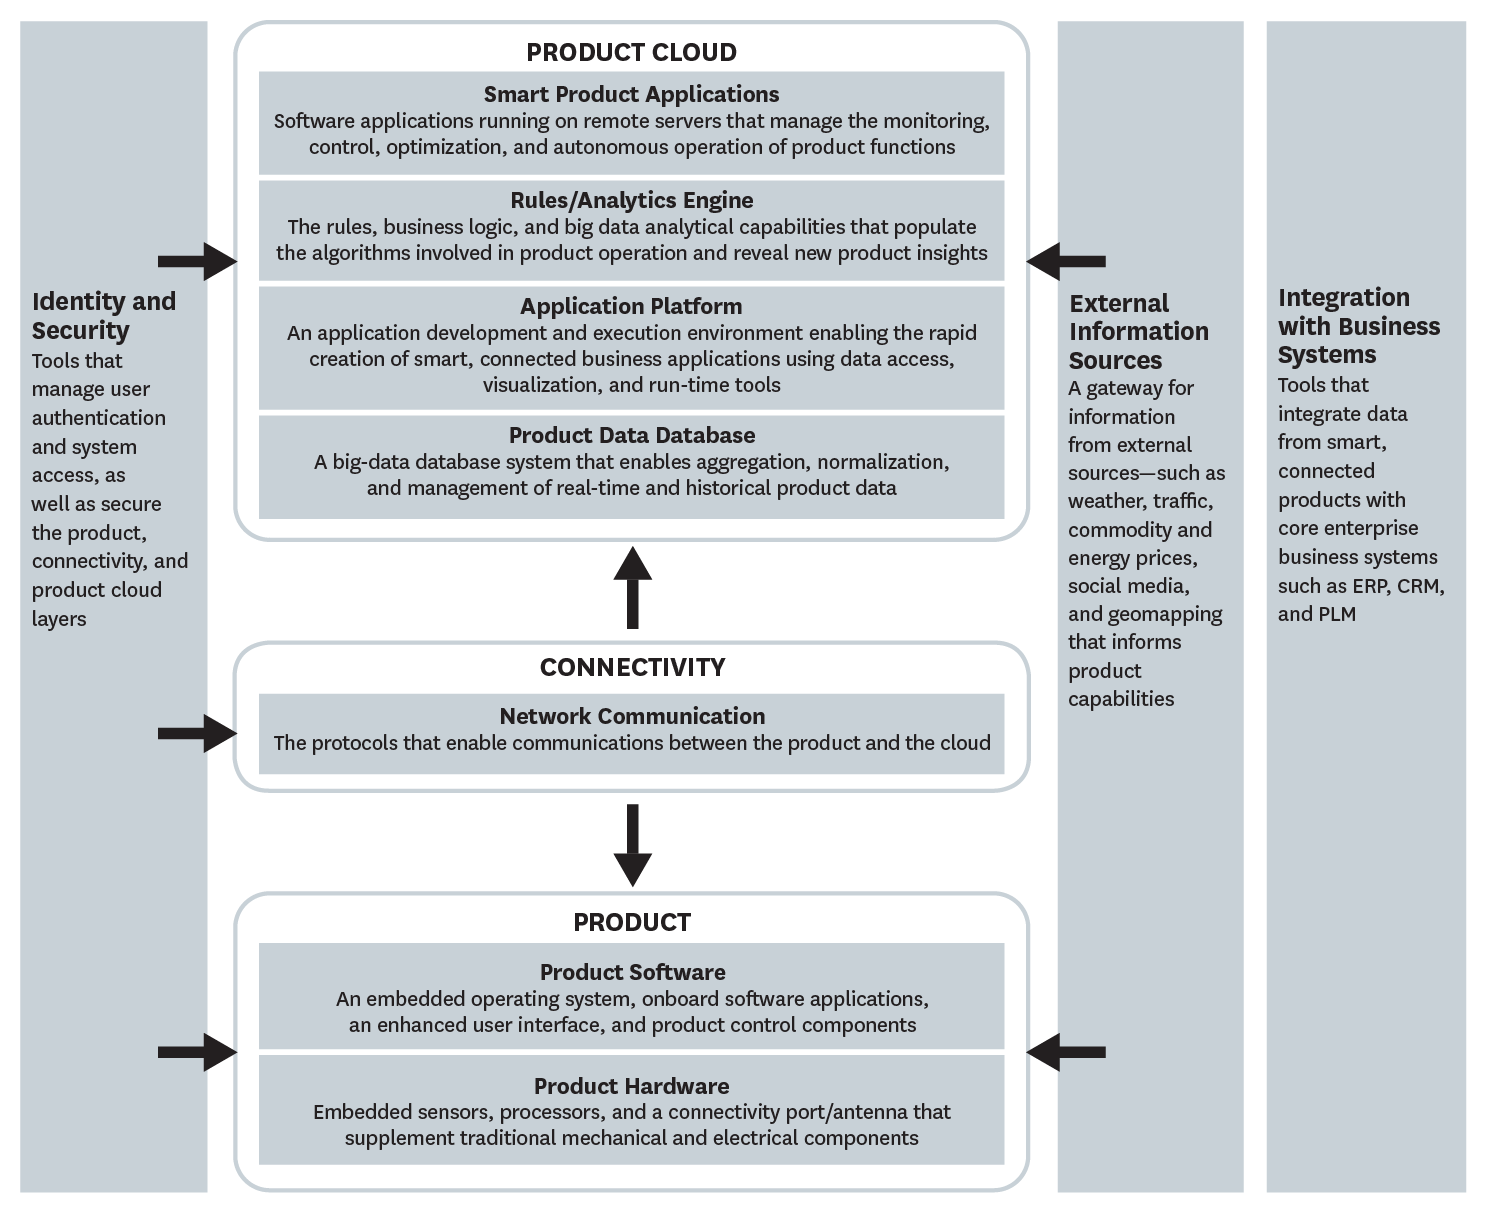
\includegraphics[width=1.1\textwidth,center]{fig/harvard_technology}
\caption{Den nye teknologistakken \citep{iot_harvard_smart}.}
\label{fig:iot_harvard_smart}
\end{figure}

\begin{figure}
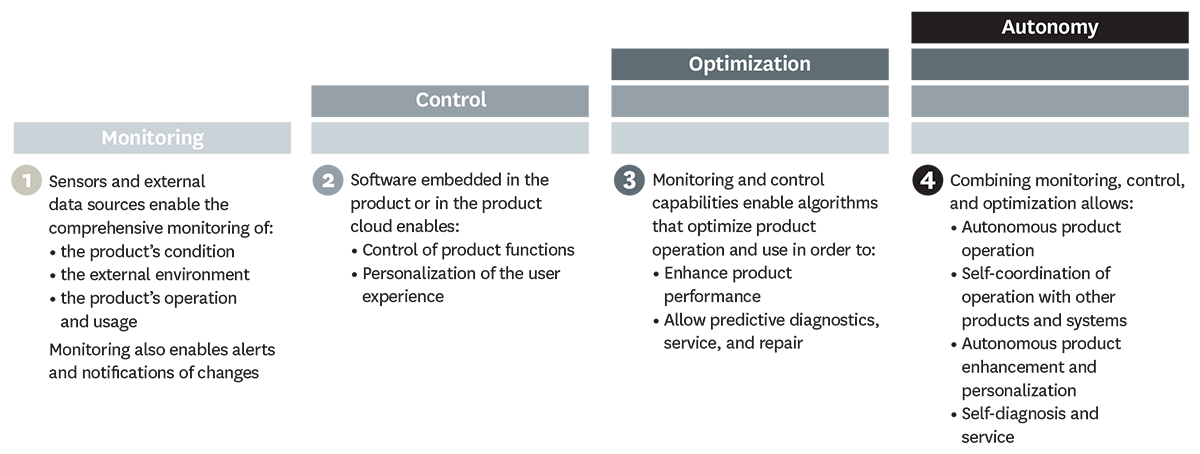
\includegraphics[width=1.1\textwidth,center]{fig/harvard_capabilities}
\caption{Egenskapene til smarte produkter \citep{iot_harvard_smart}.}
\label{fig:iot_harvard_capabilities}
\end{figure}


\subsection{Sikkerhet i tingenes internett}
Eksperter har kommet med innvendinger når det gjelder sikkerhetsmodellen til \gls{iot}.
21. oktober 2017 ble Internett-kjerneinfrastrukturselskapet \textit{Dyn} angrepet av flere millioner
små enheter (hovedsaklig rutere og kameraer) med lav grad av sikkerhet \citep{iot_attack_ddos}.
Dette påvirket flere store nettsider som Twitter, Spotify og PayPal. Rutere og webkameraer leveres
ofte med standardpassord som brukere ikke endrer selv. I tillegg til dette kan flere vanlige
porter som 22 (SSH), 80 (HTTP) og 23 (Telnet) være helt åpne mot omverdenen \citep{iot_mirai_botnet}.

\citet{iot_schneier_regulation} oppfordrer myndighetene til å pålegge restriksjoner på \gls{iot}.
Han argumenterer for at markedene selv ikke klarer å beskytte sikkerheten til forbrukerne.
Forbrukerne bryr seg ikke, produsentene bryr seg ikke og produktene kan aldri patches
etter de er solgt og levert. Denne diskusjonen om reguleringer må gjøres før det skjer
en \gls{iot}-katastrofe, mener Schneier. % @Todo: en iot-katastrofe where feelings are heated?


\section{Tingenes internett i velferdsteknologi}
Personal Connected Health Alliance (PCHA) publiserer Continua-designretningslinjene hvert år,
et åpent rammeverk for ende-til-ende-kompabilitet i personlige, tilkoblede helseenheter og helsesystemer \citep{continua_guidelines}.
En oversikt av Continua-rammeverket kan finnes i figur \ref{fig:continua}. Personlige enheter kommuniserer med
protokoller som Bluetooth eller Zigbee til en hub (Personal Area Network), og denne huben sender informasjonen
videre til et telehelse-servicesenter. Derfra kan dataen overføres til helseregisteret.

Som en del av «Omsorgsplan 2020» og nasjonalt program for velferdsteknologi, bestemte regjeringen
i slutten av 2014 at Continua-rammeverket skal være grunnlaget for alle velferdsteknologiløsninger i Norge.
Dette var også anbefalingen til Helsedirektoratet --
å standardisere på ett rammeverk sikrer at ulike løsninger virker godt sammen \citep{regjeringen_continua}.

\begin{figure}
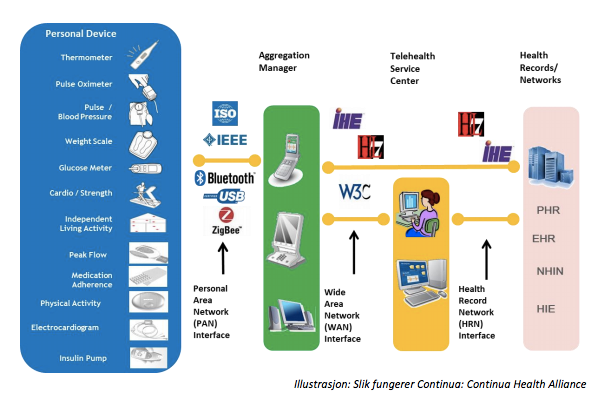
\includegraphics[width=0.9\textwidth,center]{fig/continua}
\caption{Oversikt over Continua-rammeverket}
\label{fig:continua}
\end{figure}

\chapter{Forskningsmetoder}
\label{ch:method}
Dette kapittelet redegjør for forskningsmetodene til prosjektet. Forskningsstrategiene og datagenereringsmetodene
tar utgangspunkt i \citet{oates}. Se figur \ref{fig:oates_model} for en oversikt over forskningsrammeverket.

\begin{figure}
\centering
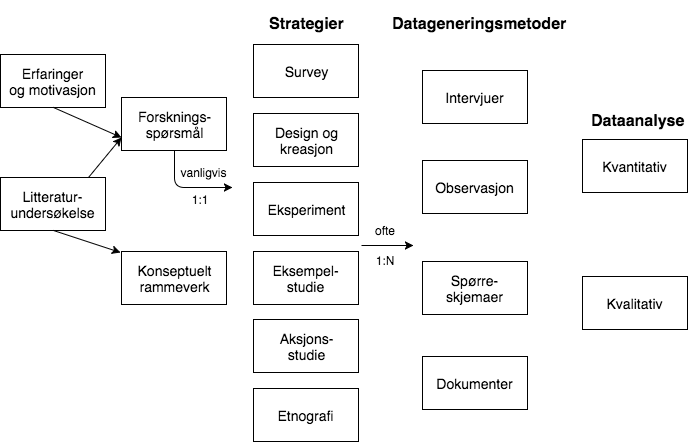
\includegraphics[width=0.90\textwidth]{fig/oates/oates_research_norwegian}
\caption{Modell av forskningsprosessen fra \citet{oates}.}
\label{fig:oates_model}
\end{figure}

\section{Forskningsstrategier}

\subsection{Design og kreasjon}
\textquote[\cite{oates}]{Forskningsmetoden design og kreasjon fokuserer på utvikling av nye IT-produkter, også kalt \textit{artefakter}.
Typer IT-artifakter inkluderer (March \& Smith, 1995): begreper, modeller, metoder og implementasjoner}{.}
Hovedpoenget er å lære gjennom å lage, og \citet{oates} identifiserer fem steg for denne prosessen:

\begin{description}
  \item[Bevisstgjøring] Hva er problemet?
  \item[Forslag] Hvordan kan problemet løses?
  \item[Utvikling] Problemløsingsfasen
  \item[Evaluering] Hvordan gikk dette?
  \item[Konklusjon] Hva kan vi trekke ut av dette?
\end{description}

\subsection{Case-studie}
Yin (2003) definerer i følge \citet{oates} case-studie som \textquote{en empirisk undersøkelse
som utforsker et samtidsfenomen i kontekst til virkeligheten, spesielt når grensene mellom fenomenet
og konteksten ikke er helt klart}{.}
\textquote[\cite{oates}]{En case-studie fokuserer på én instans av det som skal undersøkes: en organisasjon, en avdeling, et informasjonssystem,
    et diskusjonsforum (...). Denne ene instansen, eller tilfellet, studeres i detalj med forskjellige datagenereringsmetoder som
    intervju, observasjon, dokumenter (...)}{.}

Det som kjennetegner en case-studie er at det mer fokus på dybde snarere enn bredde,
at casen undersøkes i en naturlig ramme på en helhetlig måte, med flere kilder og metoder \citep[s. 142]{oates}. En undersøkende case-studie er nyttig for å kunne forstå
forskningsområdet bedre og definere gode forskningsspørsmål,
spesielt dersom det eksisterer lite forskning allerede, mens en beskrivende studie vil rette seg mer
mot å belyse én sak fra flere sider i en helhetlig historie. Den siste typen
case-studie er forklarende, og ønsker å finne ut hvorfor noe spesielt skjedde og hva
som forårsaket det \citep[s. 143]{oates}.
    
\subsection{Prototyping}

\subsection{Brukersentrert utvikling}
Brukersentrert utvikling er en prosess der brukeren er involvert i hvert steg.
Stegene er å forstå brukskonteksten, etablere krav, implementere artefakt og evaluere artefakt. Dette er en syklus som kan gjentas flere ganger.
\citet{dis20099241} standardiserer brukersentrert utvikling. Se figur \ref{fig:iso9241-210}
for de ulike stegene i prosessen.
Brukersentrert utvikling passer godt i de fem stegene som inngår i «design og kreasjon»-forskningsmetoden.

\begin{figure}
\centering
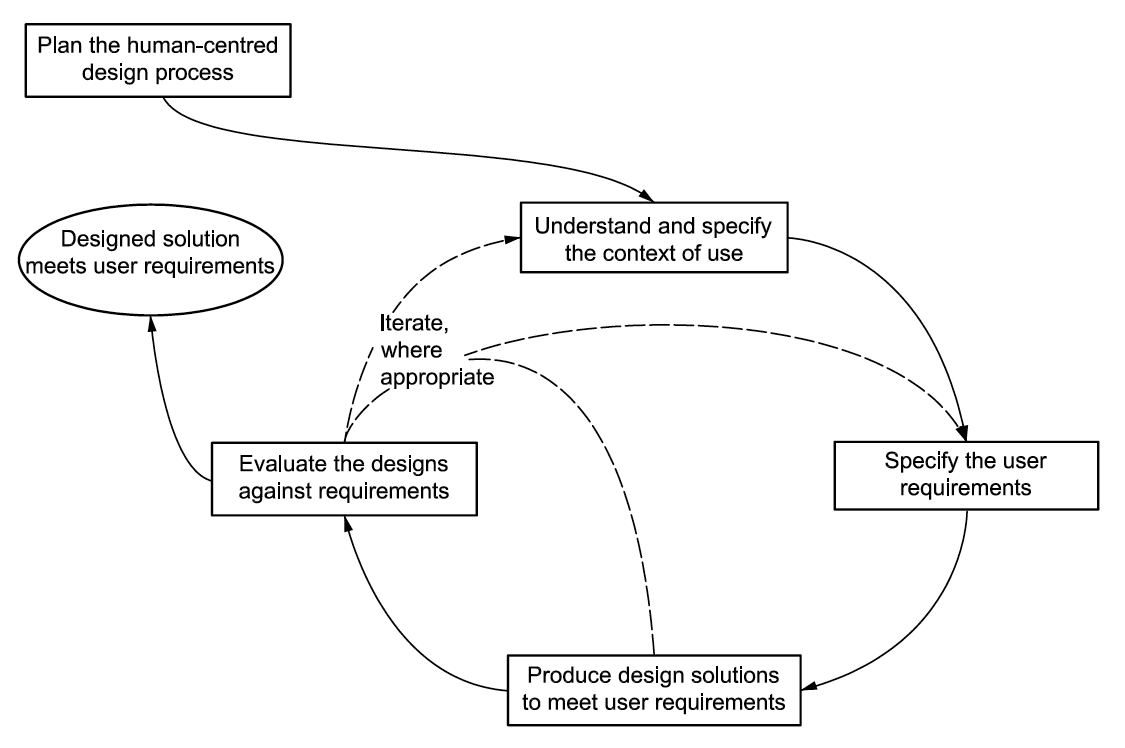
\includegraphics[width=0.85\textwidth]{fig/iso9241-210}
\caption{Gjensidige avhengigheter innenfor menneskeorientert designaktiviteter \citep{dis20099241}.}
\label{fig:iso9241-210}
\end{figure}

\section{Datagenereringsmetoder}

\subsection{Semistrukturert intervju}
Det finnes flere forskjellige typer intervju. Semistrukurert intervju er en datagenereringsmetode
der temaer og spørsmål er forberedt på forhånd, men rekkefølgen spørsmålene stilles i kan endre seg
og nye temaer og spørsmål kan komme opp basert på samtalen man har med intervjuobjektet. Det er et
kompromiss mellom et strukturert intervju og et helt ustrukturert intervju \citep[s. 188]{oates}.

Det er en mye brukt metode i case-studier for å få detaljert informasjon ut av intervjuobjektet.
I tillegg kan metoden brukes til å få tilbakemeldinger fra brukere på en kravspesifikasjon og en
endelige prototype \citep[s. 187]{oates}.

\subsection{Dokumenter}

\chapter{Forskningsdesign}
\label{ch:design}

I dette kapittelet presenteres og drøftes forskningsdesignet til studien.
I tillegg diskuteres tilliten og troverdigheten til forskningen. 
Som nevnt tidligere, bygger rammeverket til forskningsprosessen på boken
\textit{Researching Information Systems and Computing} \citep{oates}.

\iffalse
I en forskningsartikkel er avsnittet om metode ofte det viktigste. Det samme gjelder metodekapitlet i en empirisk oppgave. Dette kan også være et vanskelig kapittel å skrive, fordi det ikke alltid er klart hvilken «jobb» det skal gjøre. Et metodekapittel skal ikke gjengi innholdet i fagets metodebøker. Dersom du har brukt intervju er det for eksempel ikke nødvendig å liste opp forskjellige typer forskningsintervju. Du trenger heller ikke redegjøre for forskjellene mellom kvantitative og kvalitative metoder, eller liste opp ulike typer validitet og reliabilitet.

Det du skal gjøre, er å vise hvordan dine valg av design og metode egner seg til å belyse/besvare ditt forskningsspørsmål, og hvilke vurderinger du har foretatt mht validitet (gyldighet) og reliabilitet (pålitelighet).’Show, don’t tell’ – vis leseren hva du gjorde, og forklar hvorfor. Da vil metodekapitlet sette de ulike delene av oppgaven i sammenheng, og det blir spennende å lese. I praksis betyr dette å demonstrere at du har forstått den praktiske betydningen av begrepene.

Et godt metodekapittel forteller hva du har gjort i din undersøkelse, og forklarer hvorfor. Hvordan samlet du inn data? Hva kan man forvente å finne ved å gjøre det på denne måten?
Hva var rammene? Hvilke avveininger måtte tas? Hva oppnår du ved å bruke denne metoden?
Vis hva du har gjort for å øke validiteten. Hva kan du si om reliabiliteten (påliteligheten) i datainnsamlingen? Hvordan vet du at du har undersøkt det du ønsket å undersøke? Hvilke slutninger kan trekkes på dette grunnlaget? Hvilke slutninger er sikre, og hvilke er mer tentative? Hvilken overføringsverdi har resultatene? Kan du generalisere – hvorfor, hvorfor ikke?
Svakheter og styrker ved metoden skal beskrives. Den ekstra gode oppgaven utmerker seg ved å forsvare sine valg og samtidig kritisere dem.

Formål
Produkter (bidrag/resultater)
Prosess
Deltakere
Paradigme
Presentasjon
\fi

\section{Forskningsspørsmål}
Som skrevet i kapittel \ref{ch:introduction}, er formålet med denne forskningen å undersøke hvordan ny teknologi basert
på \gls{iot}-skyløsninger kan brukes til avstandsoppfølging med prosjektet til Trondheim kommune som ramme:
\textbf{«\fs{}»}

Forskningsspørsmålene som ligger til grunn for denne masteroppgaven har gått igjennom en iterativ prosess i løpet av arbeidet
med oppgaven. Det vil si at intervjuene gjort med Trondheim kommune og arbeidet med den tekniske løsningen har påvirket
det prosjektet ønsker å undersøke nærmere. Alle forskningsstrategiene utdypes nærmere i delkapittel \ref{sec:forskningsstrategier}.

\subsection{Forskningsspørmål 1}
\textbf{\fs{1}}

Avstandsoppfølging er ganske nytt i Norge, og det foreligger ikke så mye informasjon om hvordan det gjøres ettersom
det i skrivende stund fortsatt er i testfasen i mange kommuner. Trondheim kommune vil bli brukt som et eksempel på hvordan avstandsoppfølging
gjøres i dag og hvilke planer de har for ny teknologi i tiden som kommer.

For å belyse spørsmålet er forskningsløpet som i figur \ref{fig:oates_fs1}. Case-studie er hovedstrategien, og intervjuer og dokumenter
er datagenereringsmetodene.

\begin{figure}
\centering
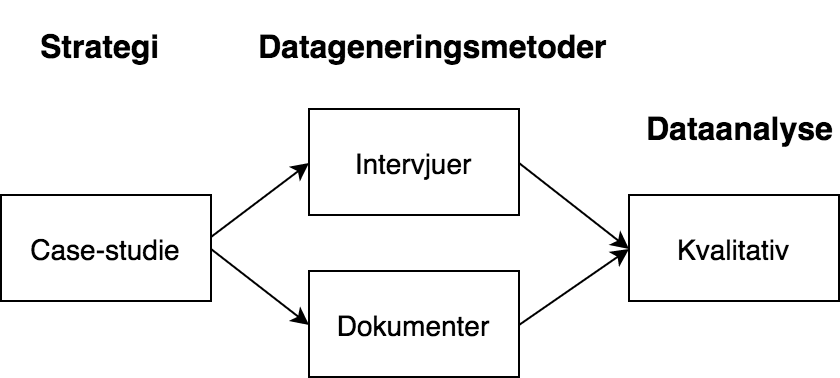
\includegraphics[width=0.65\textwidth]{fig/oates/fs1}
\caption{Forskningsstrategien til FS1}
\label{fig:oates_fs1}
\end{figure}

\subsection{Forskningsspørmål 2}
\textbf{\fs{2}}

Hovedstrategien er design og kreasjon, med intervjuer og dokumenter som datagenereringsmetode (figur \ref{fig:oates_fs2}). Ved å lage
et \textit{proof of concept} basert på eksisterende skyteknologi, er målet å finne en mulig teknologistakk. Case-studien av Trondheim
kommune hjelper til med å forstå brukskonteksten og kravene til en slik teknologistakk.

Teknologistakk er definert
som klientsiden av applikasjonen, hvordan denne snakker med sensorene rundt -- og på hvilken måte sensordataene sendes og behandles av
en bakenforliggende serverløsning.

\begin{figure}
\centering
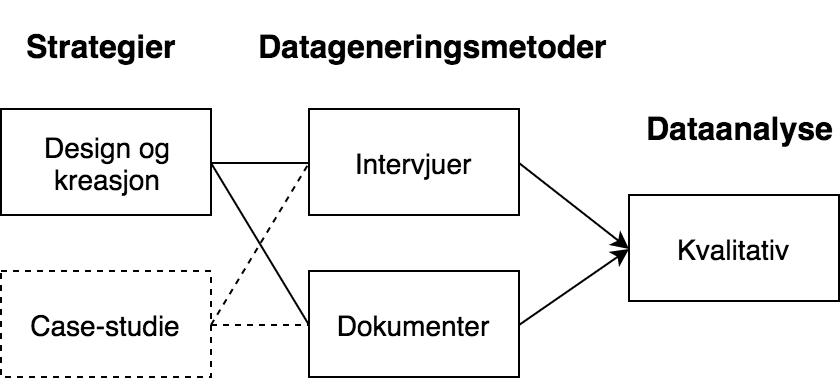
\includegraphics[width=0.65\textwidth]{fig/oates/fs2}
\caption{Forskningsstrategien til FS2}
\label{fig:oates_fs2}
\end{figure}
    
\subsection{Forskningsspørmål 3}
\textbf{\fs{3}}

Forskningsstrategien er å lage en frittstående løsning i form av et skytilkoblet pulsoksymeter og evaluere
denne løsningen med semistrukturerte intervjuer (figur \ref{fig:oates_fs3}).
 
Frittstående betyr at løsningen er helt plattformuavhengig og ikke basert på eksisterende plattformer som Android og iOS.
Domeneeksperter er definert som forskere og prosjektledere innenfor velferdsteknologi og avstandsoppfølging.

\begin{figure}
\centering
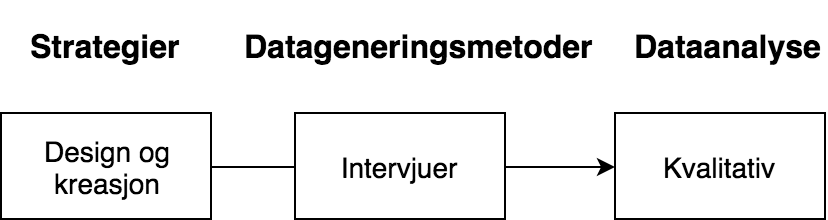
\includegraphics[width=0.65\textwidth]{fig/oates/fs3}
\caption{Forskningsstrategien til FS3}
\label{fig:oates_fs3}
\end{figure}

\subsection{Forskningsspørmål 4}
\textbf{\fs{4}}

Dette forskningsspørsmålet sammenstiller all data fra de andre forskningsspørsmålene. Det søker å finne ut hva implikasjonene
er for utviklingen av skybasert \gls{iot} for avstandsoppfølging gjennom en kvalitativ analyse og drøfting.
Figur \ref{fig:oates_fs4} oppsummerer hele forskningsløpet.

\begin{figure}
\centering
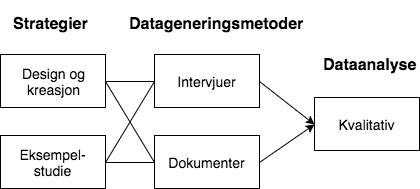
\includegraphics[width=0.65\textwidth]{fig/oates/fs4}
\caption{Forskningsstrategien til FS4}
\label{fig:oates_fs4}
\end{figure}

\section{Forskningsstrategier}
\label{sec:forskningsstrategier}
Dette delkapittelet drøfter kort fordelene og ulempene til forskningsstrategiene som er valgt.

\subsection{Design og kreasjon av et pulsoksymeter}
I følge \citet[s.121-122]{oates} er fordelene til design og kreasjon-strategien at det er enklere å relatere til noe
som eksisterer i virkeligheten enn en íde, en tanke eller et konsept.
Den raske teknologiutviklingen gjør også at det er mulig å foreslå og utvikle nye artefakter, og at man dermed bidrar til ny kunnskap.

Ulempen med å velge denne strategien er at det er fort gjort at en kun demonstrerer
teknisk kompetanse uten at det kvalifiserer som god forskning. I tillegg til det nye produktet må ny kunnskap utvikles, bygget
på analyse, argumenter og kritiske evalueringer \citep[s. 109]{oates}. En ting er at det lages et nytt produkt i et domene --
viktigere momenter er hvilken ny informasjon den fører med seg og konteksten den blir satt inn i.

Artefakten i dette prosjektet er en høynivå prototype i form av et proof of concept, både på hardware- og softwaresiden.
Siden teknologiutforsking er et mål, vil
prototypen implementeres, og ikke være en lavnivå papirprototype. Den industrielle utformingen av prototypen vektlegges ikke. Det er
ikke meningen at prototypen skal ut i produksjon slik som den er designet. En annen tilnærming kunne vært å vektlegge brukerperspektivet enda mer,
og gjennomføre flere runder med brukertester med helsepersonell og pasienter. Brukertester med pasienter ville medført krav om
riktig behandling av sensitive helseopplysninger og en godkjent søknad til Norsk senter for forskningsdata (NSD).

Brukersentrert utvikling er metodikken som brukes for design og kreasjon av prototypen. Filosofien bak å inkludere brukeren i hvert aspekt
av utviklingen er å fortere finne ut hva som ikke fungerer slik at en ikke maler seg inn i et hjørne. Case-studien av avstandsoppfølging
i Trondheim kommune hjelper til med å forstå konteksten pulsoksymeteret skal brukes i og hvordan det skal brukes, noe
som fører til at utviklingen av en prototype blir enklere.

\begin{minipage}{\linewidth}
Dette er design og kreasjon-strategien oppsummert:\newline

\begin{description}
  \item [Bevisstgjøring] Semistrukturert intervju med Trondheim kommune om velferdsteknologi og avstandsoppfølging. Kort bakgrunnkapittel
      om velferdsteknologi og avstandsoppfølging (kapittel \ref{ch:background}).
  \item [Forslag] En frittstående og skytilkoblet velferdsteknologiløsning der sensorene er innebygget vil fungere bedre
      eller like bra som eksisterende løsninger med nettbrett.
  \item [Utvikling] En prototype av et skytilkoblet pulsoksymeter med fingeravtrykksensor som autentiseringsmetode.
  \item [Evaluering] Semistrukturerte intervjuer med Trondheim kommune og SINTEF der prototypen vises fram.
  \item [Konklusjon] Baseres på alle de foregående stegene.
\end{description}
\end{minipage}

Hvordan evalueringen av prototypen med semistrukturerte intervjuer ble gjennomført er beskrevet i kapittel \ref{ch:evaluation1}.

\subsection{Case-studie: Avstandsoppfølging i Trondheim kommune}
Det er flere tilnærminger til avstandsoppfølging, og det er flere kommuner enn Trondheim som har pågående forsøk, blant annet
Sarpsborg og Oslo. Fordelen med å velge ut én kommune er at det belyser hvordan de har tilnærmet seg avstandsoppfølging
som helhet og forenkler datainnhentingen -- det er naturlig å velge ut Trondheim kommune siden det gjør tilgangen på personer er bedre.

Ulemper med denne strategien er, i følge \citet{oates}, at mangelen på streng krav kan føre til generaliseringer med
lav kredibilitet, at det kan være
vanskelig å få tilgang til riktige personer og riktig informasjon, samt at forskeren i seg selv kan påvirke mye av det som blir gjort fordi det er
så få regler. Målet med case-studien er å skjønne hvilke problemstillinger Trondheim kommune prøver å løse, hvordan de løser det og hvilke
erfaringer de har gjort seg hittil. Dette vil påvirke den nye teknologien som bygges i dette forskningsprosjektet.

Datageneringsmetoder i dette case-studiet er semistrukturerte intervjuer og dokumenter. Observasjon av hvordan pasientene bruker Trondheim kommunes løsning
kunne vært en god metode, men for å snevre inn omfanget og slippe å innhente tillatelser velges ikke denne metoden. Det hadde vært mer
aktuelt om case-studiet hadde vært den eneste hovedstrategien i prosjektet. Eksempler på dokumenter er all den informasjonen som finnes om
avstandsoppfølging på Internett og det Trondheim kommune har lagt ut selv. Helsedirektoratet og Datatilsynet
har også en rekke retningslinjer og råd som kommunene må og kan forholde seg til.

Hvordan de ulike intervjuene ble gjennomført og analysert er beskrevet i starten av kapittel \ref{ch:case}.

\section{Forskningsparadigme og forskningskvalitet}
Forskningsprosjektet inneholder kun kvalitative datagenereringsmetoder, og er dermed en form for kvalitativ forskning.
Det tar en interpretivistisk tilnærming til det som skal undersøkes. Det er flere måter å gjøre avstandsoppfølging på,
og det er ikke sikkert at en metode er bedre enn en annen.
Siden kun kvalitativ data analyseres, vil nødvendigvis forskerens subjektive holdninger påvirke drøftingen av forskningsspørsmålene.

Validitet og objektivitet må forstås på en annen måte i dette prosjektet enn om dette for eksempel hadde vært et
kvantitativt eksperiment. Lincoln og Guba foreslår, i følge \citet{oates},
at kriteriene for interpretivisme
heller skal være hvor stor tillit man kan ha til forskningen, gjennom begrepene bekreftbarhet, pålitelighet, troverdighet og overførbarhet.
Her handler bekreftbarhet og pålitelighet om hvorvidt studiet er godt nok beskrevet og dokumentert til at man skjønner hvordan det har
foregått og kan stole
på forskningsløpet. Forskning blir mer troverdig med flere forskjellige kilder til data og om man sjekker med kildene om man har
tolket data riktig.

\subsection{Bekreftbarhet og pålitelighet}
Tidligere i kapittelet er fremgangsmåten til studiet presentert. All kode ligger åpent tilgjengelig på Internett slik at hvem som helst kan
titte på den. Transkriberinger av intervjuene er tilgjengelige ved forespørsel. Senere vil implementasjonen av prototypen beskrives i
så god detalj at det er mulig å lage noe tilsvarende kun ved å lese i teksten og se på koden.

\subsection{Troverdighet}
Alle intervjuene med Trondheim kommune må tolkes med det faktum at prosjektlederne har en tilknytning som
gjør at de ønsker at avstandsoppfølgingprosjektet
skal lykkes i bakhodet. Aktører direkte involvert i et prosjekt er mottakelige for bekreftelsestendenser der man søker etter å bekrefte noe
man allerede tror. Selv om SINTEF er en tredjepart som bistår Trondheim kommune, er de også mye involvert i prosjektet.
Det er mulig at forskningen kunne blitt enda mer troverdig med en kritisk tredjepart uten direkte tilknytning til velferdsteknologiprosjektet i Trondheim.
Gjerne en stemme som ikke er udelt positiv til avstandsoppfølging som teknologi for velferd.
Fordelen med å snakke med personer som jobber med avstandsoppfølging i Trondheim kommune, er at de har veldig god kunnskap om temaet
og muligheten til å sammenligne løsningen som presenteres i denne forskningen med noe som eksisterer i praksis i dag.
De er en troverdig stemme i avstandsoppfølgingdebatten.

\subsection{Overførbarhet}
Spørsmålet som må stilles er om funnene og arbeidet gjort i dette prosjektet kan overføres til avstandsoppfølging som generelt tilfelle.
Trondheim kommune brukes som eksempel, og konklusjonen vil generalisere med kun dette tilfellet som bakgrunn.
Er det faktisk mulig å finne noen implikasjoner for utviklingen av skybasert \gls{iot} som teknologisk plattform for avstandsoppfølging?
Hvilke resonnementer og argumenter er i så fall disse resonnementene fundert i? Prosjektets overførbarhet vil diskuteres i
kapittel \ref{ch:discussion}.

% @Todo ??? 
% Det som taler for at man kan det er at
% Det som taler mot er at 

\chapter{Case-studie: Avstandsoppfølging i Trondheim kommune}
\label{ch:case}

\section{Innsamling av data}
Materialet i dette kapittelet er hovedsaklig basert på et gruppeintervju gjort med Renate Enger og Ingar Børre Sandvik med besøk
av en fastlege. Dette intervjuet ble gjennomført 24. mars 2017 fra kl. 09.00 til kl. 10.50 i lokalene til Trygghetspatruljen i
Trondheim kommune i Klæbuveien. Den formelle henvendelsen til velferdsteknologiprogrammet i Trondheim kommune er vedlagt i
tilegg \ref{appendix:formell}, og intervjuhendelsen er vedlagt i tillegg \ref{appendix:invitasjon_evaluering}. Temaene og
de forhåndsskrevne spørsmålene til intervjuet ligger i vedlegg % @TODO: legg til intervjuguide i vedlegg
Noe materiale fra evalueringsintervjuene gjort med SINTEF og Trondheim kommune i mai er
også med. Hvordan disse intervjuene ble gjennomført er nøyere beskrevet i kapittel \ref{ch:evaluation1}.

Trondheim kommune ga forskningsprosjektet en bruker til testmiljøet til løsningen de kjører. De viste også fram
nettbrettet som brukerne får utdelt. Dette, og informasjonen som allerede ligger tilgjengelig på nettet er en del
av dokumentdelen som analyseres.

\section{Bakgrunn og tjenesteforløp}
I følge I. B. Sandvik (personlig kommunikasjon, 24. mars, 2017), ble Trondheim kommune valgt ut til å delta i avstandsoppfølgingsprosjektet hovedsaklig fordi de hadde et
prosjekt tidligere som het \textit{HelsaMi} der ti KOLS-pasienter ble fulgt opp hjemme. I dette prosjektet var det ikke noen sensorer involvert,
kun mulighet til å rapportere dagsform med et nettbrett.

Trondheim kommune drifter de fleste tjenestene som for eksempel hjemmebesøk, helsevakta, avstandsoppfølging og responssenter med egne ressurser:
\textquote[I. B Sandvik, 24. mars, personlig kommunikasjon]{Trondheim kommune har jo en veldig tydelig politisk ledelse og forankring på å ha mesteparten av
    ansvaret for sin egne tjenester selv, altså inhouse}{.}
Dette skiller seg fra Oslo og Sarpsborg som har større grad av outsourcing av tjenestene. Han påpeker også at Trondheim kommune til dels skiller
seg fra andre kommuner ved å tenke på robuste tjenester som helhet, og ikke bare på teknologien:
\blockquote[I. B Sandvik, 24. mars, personlig kommunikasjon]{For det som Trondheim kommune er
    veldig tydelige på, og kanskje til dels skiller oss fra andre kommuner når det gjelder velferdsteknologi -- det er at det er ikke teknikken og dingsene som på en måte skal
    løse alt. Det er tjenesten vi skal bygge som understøttes av teknologien.
    Vi ser jo det at det å kunne pilotere i småskala, med ny teknologi, det greier de fleste. Men det å bygge en robust tjeneste som skal implementeres i en stor kommune
-- det er noe helt annet. Og som skal da kunne rulles ut i storskala med mange hundre brukere av ulike tjenester.}

\section{Eksisterende løsning}
Brukeren har et nettbrett som kjører en androidapplikasjon. Denne applikasjonen pakker inn
et webgrensesnitt. I tillegg til hovedapplikasjonen er det en sensorhub-applikasjon som kjører i bakgrunnen
og har ansvaret for tilkoblingen til alle sensorene. Alle skjermbildene i dette delkapittelet er tatt i testmiljøet
til Trondheim kommune i en nettleser.

Beskrivelsen av løsningen og skjermbildene tar utgangspunkt i to scenarioer for sluttbrukere
og ett scenario for helsepersonell: for brukere er det å rapportere dagsform og utføre en måling med pulsoksimeter,
og for helsepersonell er det å gå inn for å se på hvilken data som er kommet inn.

Det første som møter brukeren er hovedskjermen i figur \ref{fig:helsami_hovedskjerm}. I testmodus er alle de ulike
alternativene vist.
Herfra kan brukeren trykke seg inn for å rapportere dagsform for \textit{KOLS} og \textit{HJERTESVIKT}, eller utføre en sensormåling med
enten vekt, blodtrykk eller pulsoksimeter. Det er også mulig å gå på \textit{Brukerveiledninger} for å få instruksjoner og hjelp.
For en bruker som har KOLS og en sensor utplassert hjemme, vil skjermen for eksempel vise KOLS og SpO2.

\begin{figure}
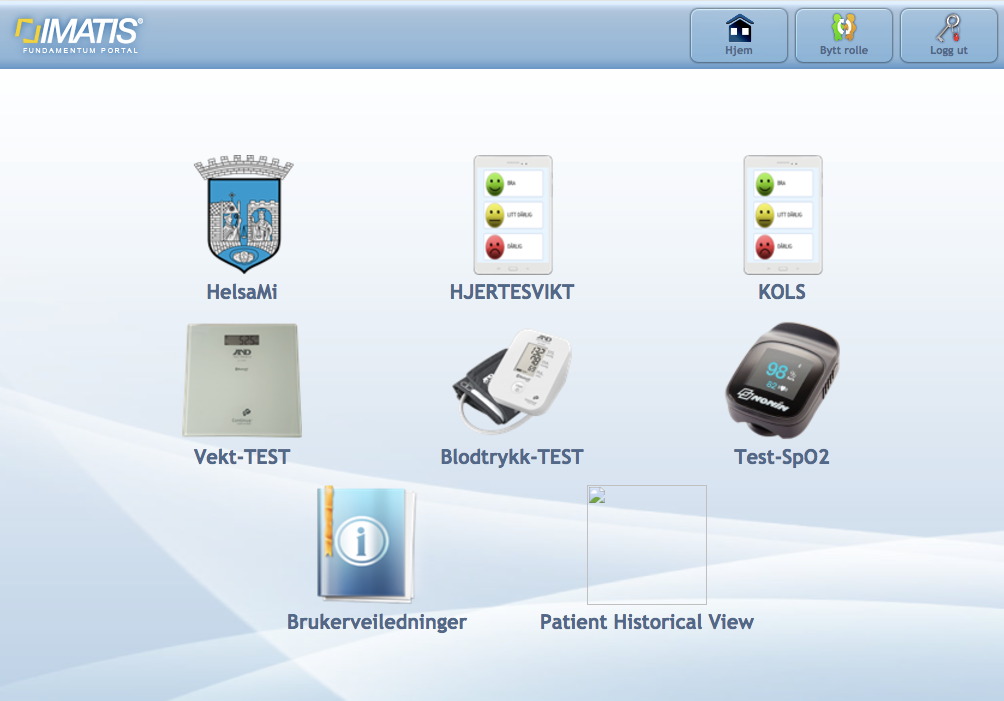
\includegraphics[width=1.0\textwidth,center]{fig/helsami/hovedskjerm}
\caption{HelsaMi+: Hovedskjerm}
\label{fig:helsami_hovedskjerm}
\end{figure}

\subsection{Rapportere dagsform}
Scenariet er at en bruker med KOLS skal rapportere dagsform. Brukeren trykker på KOLS på hovedskjermen,
og kommer til figur \ref{fig:helsami_kols_start}. Et klikk på \textit{Start} tar brukeren til \ref{fig:helsami_kols_sp1}.
Det er fire spørsmål brukeren svarer på. Alle svaralternativer som er subjektive spør brukeren om å sammenligne med
hvordan det er til vanlig.

\begin{itemize}
  \tightlist
  \item Hvordan er pusten din?
  \item Hvordan er hosten?
  \item Hvordan er fargen på oppspyttet ditt?
  \item Hvordan føler du deg til sinns?
\end{itemize}

Etter spørsmålene får brukeren mulighet til å legge inn en skriftlig kommentar og se over at det er greit
før alt sendes inn (figur \ref{fig:helsami_kols_sammendrag}). Brukeren får beskjed om at tilbakemeldingen er sendt,
og må selv aktivt klikke seg tilbake til menyen etterpå.

\begin{figure}
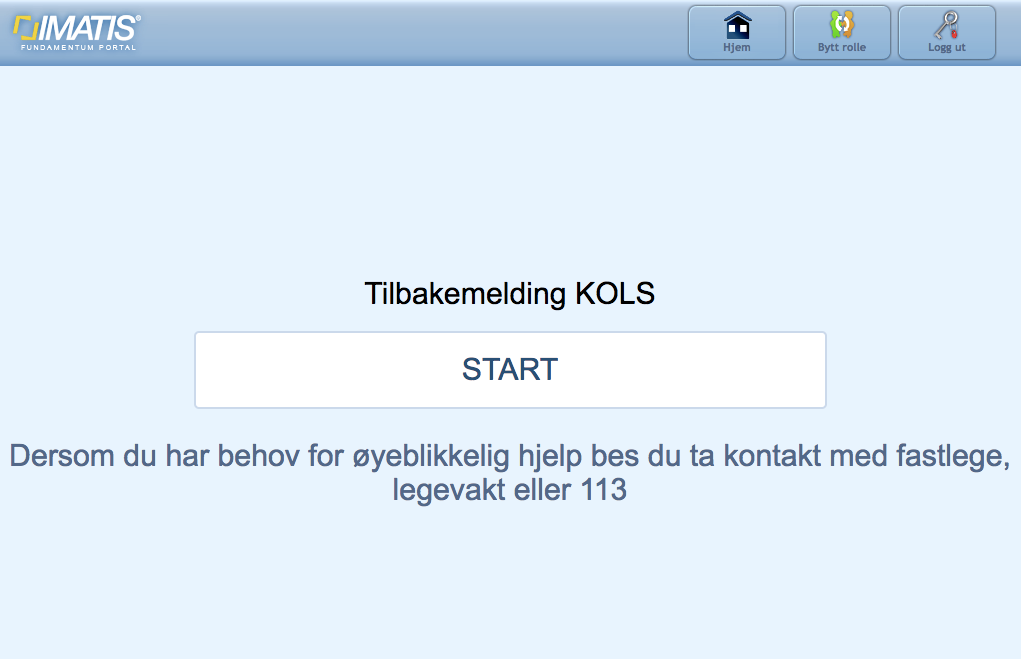
\includegraphics[width=1.0\textwidth,center]{fig/helsami/kols_start}
\caption{HelsaMi+: Tilbakemelding KOLS}
\label{fig:helsami_kols_start}
\end{figure}

\begin{figure}
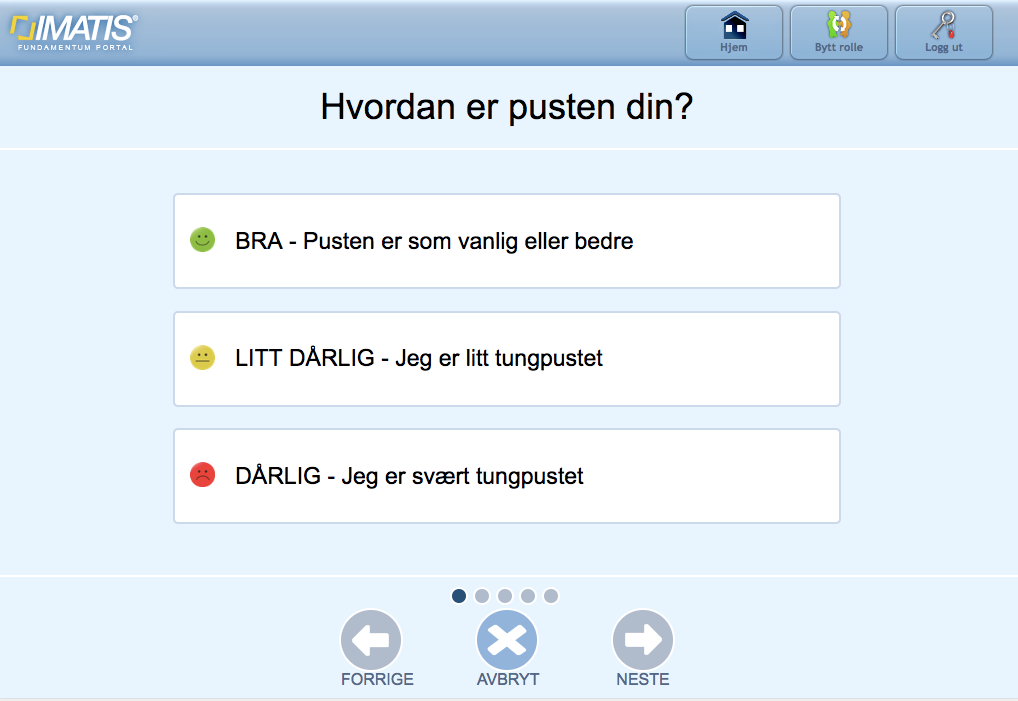
\includegraphics[width=1.0\textwidth,center]{fig/helsami/kols_sp1}
\caption{HelsaMi+: Spørsmål 1}
\label{fig:helsami_kols_sp1}
\end{figure}

\begin{figure}
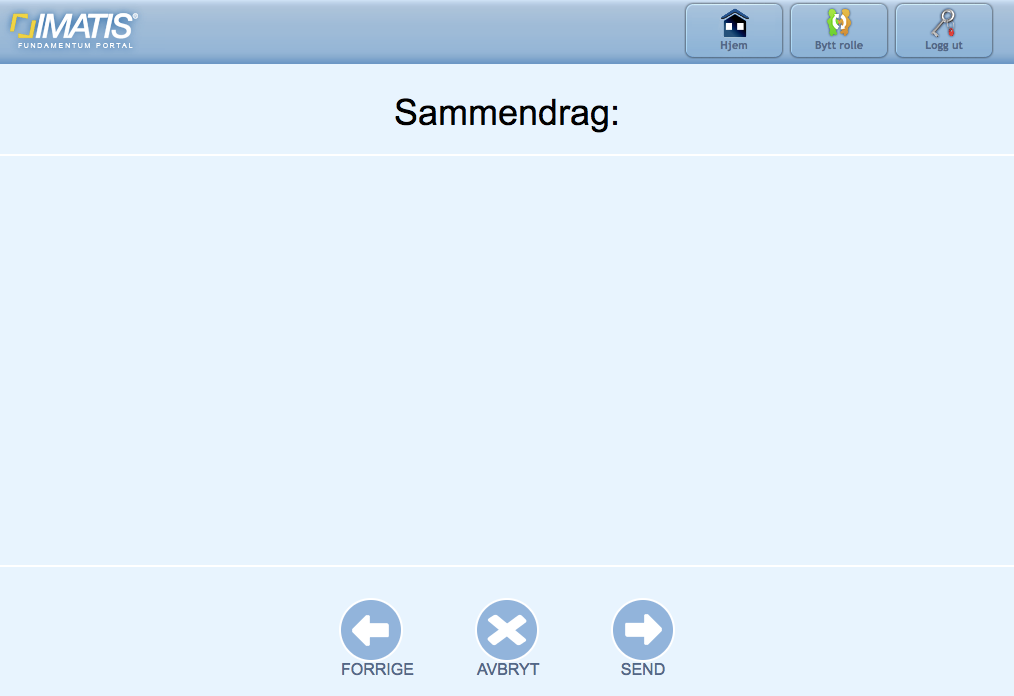
\includegraphics[width=1.0\textwidth,center]{fig/helsami/kols_sammendrag}
\caption{HelsaMi+: Sammendrag}
\label{fig:helsami_kols_sammendrag}
\end{figure}

\subsection{Utføre en måling med pulsoksimeter}
Et klikk på \textit{Test-SpO2} tar brukeren til en mellomskjerm med informasjon om at
brukeren ikke har utført en måling ennå med et bilde av sensoren. Brukeren klikker seg videre
til en skjerm med to valg, enten \textit{Trykk her for å måle oksygenmetning og puls} eller \textit{Trykk her for brukerveiledning}
(figur \ref{fig:helsami_pulsoksimeter_oversikt}). Det første valget tar brukeren til figur \ref{fig:helsami_pulsoksimeter_maaling}
der brukeren klikke på en knapp og setter måleren på fingeren. Brukeren må ha en gyldig sensorhub installert for
å få lov til å gjennomføre en måling.

\begin{figure}
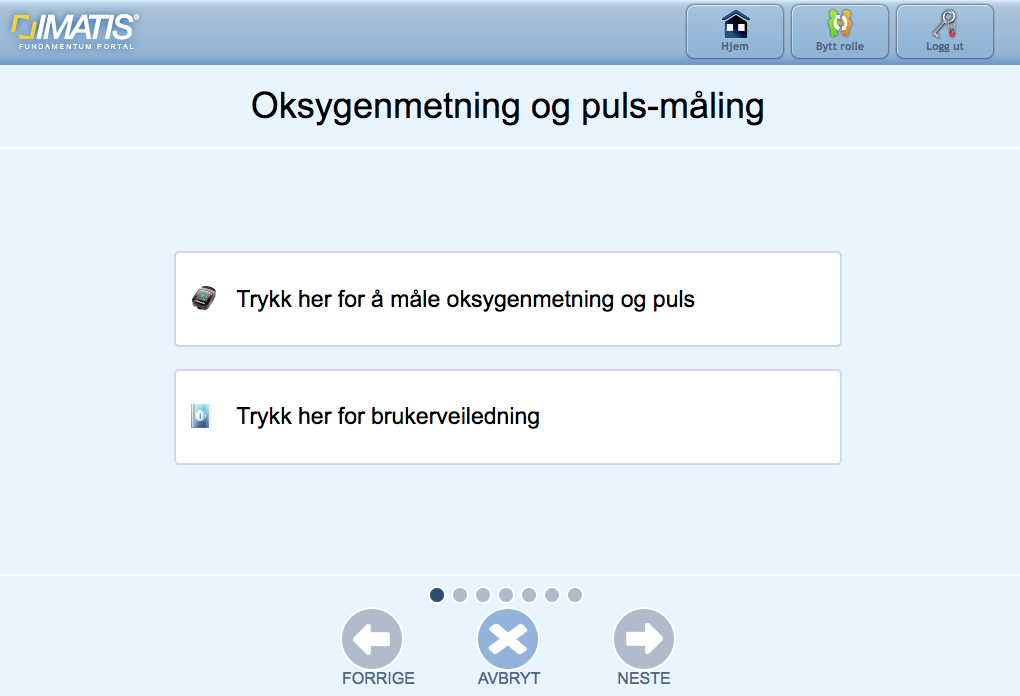
\includegraphics[width=1.0\textwidth,center]{fig/helsami/pulsoksimeter_oversikt}
\caption{HelsaMi+: Pulsoksimeter-oversikt}
\label{fig:helsami_pulsoksimeter_oversikt}
\end{figure}

\begin{figure}
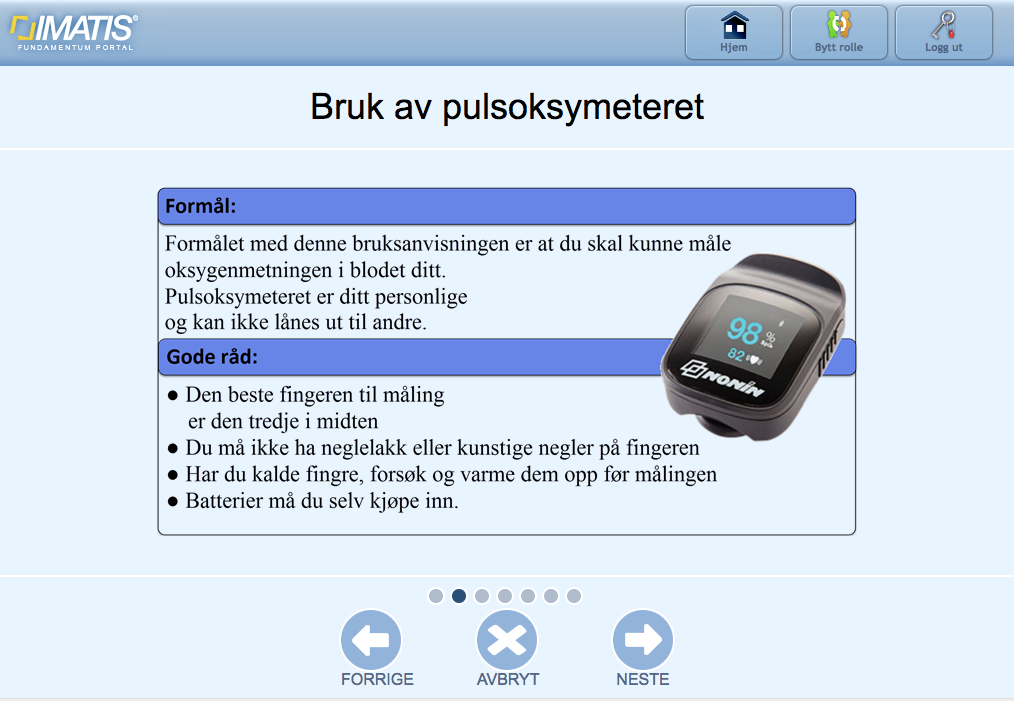
\includegraphics[width=1.0\textwidth,center]{fig/helsami/pulsoksimeter_veiledning}
\caption{Pulsoksimeter-veiledning}
\label{fig:helsami_pulsoksimeter_veiledning}
\end{figure}

\begin{figure}
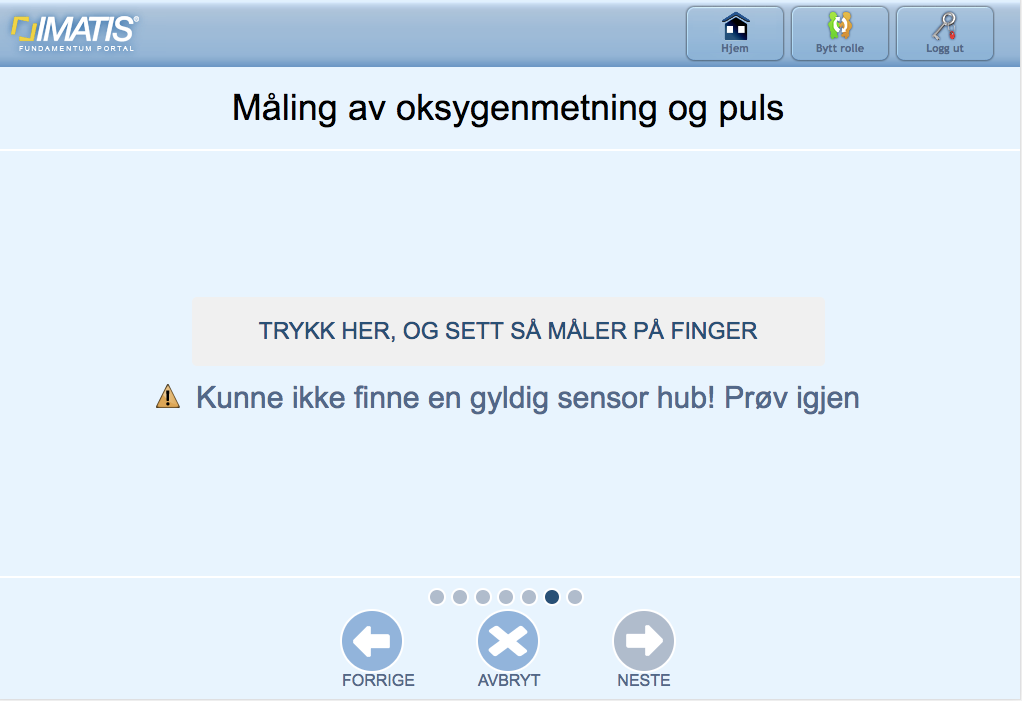
\includegraphics[width=1.0\textwidth,center]{fig/helsami/pulsoksimeter_maaling}
\caption{HelsaMi+: Pulsoksimeter-måleskjerm}
\label{fig:helsami_pulsoksimeter_maaling}
\end{figure}

\subsection{Se på innrapport data}
Trykk på \textit{HelsaMi}. Figur \ref{fig:helsami_admin1} viser hvordan oversikten over innrapportert data ser ut.

\begin{figure}
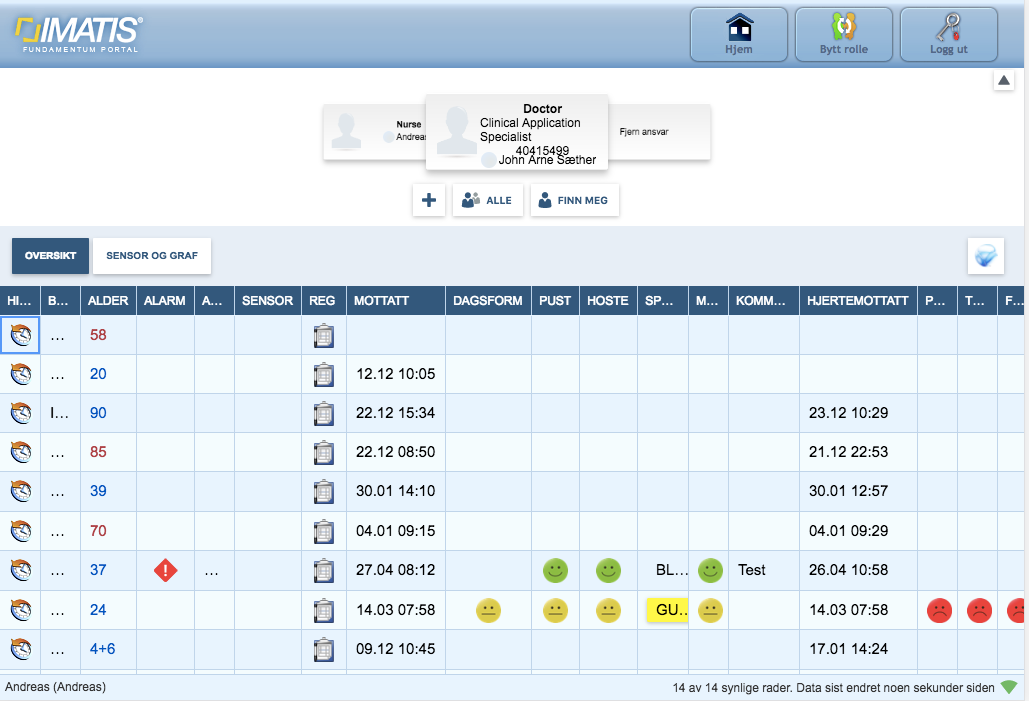
\includegraphics[width=1.0\textwidth,center]{fig/helsami/admin_oversikt}
\caption{HelsaMi+: Oversikt for administrator 1/2}
\label{fig:helsami_admin1}
\end{figure}

\section{Utfordringer og refleksjoner}
I. B Sandvik (personlig kommunikasjon, 23. mars, 2017) påpekte at den største utfordringen med prosjektet ikke er teknologien, men samhandlingen mellom de ulike
helseinstansene:

\blockquote{Det som er interessant med denne uttestingen av tjenesten er jo å se hvilke gevinster, for det er jo gevinster man ønsker å kartlegge, hvilke gevinster man tror
    man kan få med å drive med den type ny helsetjeneste med oppfølging av brukere mens de bor hjemme. og det som gjør prosjektet her så relativt komplekts -- en ting
    er jo den teknologiske delen -- det er jo stort sett håndterbart. Dette er jo et prosjekt som går på tvers av kommune, fastlege og spesialisthelsetjeneste. Det vil
si midt inne i samhandlingsreformdomenet.}

De ulike helseinstansene har forskjellige former for måloppnåelse og egne budsjetter. De statlige helseforetakene har ansvaret for sykehusene,
ikke kommunen. I. B Sandvik forklarer hvorfor dette kan være en utfordring:

\blockquote{Det er jo en utfordring av mange grunner. Både på grunn av kultur, fokus. Spesialister er jo diagnoserettet, kommunen har jo det hele mennesket som fokus. Og
    fastlegen sitter jo der i mellom og skal egentlig ha ansvaret og kontroll over alt som foregår over sine pasienter mens de er utenfor sykehuset sitt domene. Så det er
    mange interessante problemstillinger som har blitt avdekket. Blant annet det vi kan nevne et par eksempler det med det juridiske: hvem skal ha ansvaret for hva,
    hvordan skal opplysninger deles mellom partene -- ikke rett frem. Det andre er dette med finaniseringsmodellene. Det er jo ikke noe tvil om at den største investeringen
    i denne type tjeneste gjøres av kommunen, når det gjelder å rigge tjeneste, oppfølging, utstyr, alt dette her. Mens gevinstene kanskje i større
grad tas ut på sykehuset, med færre innleggelser.}

\chapter{Kvalitetskrav til løsning}
\label{ch:requirements}

Kvalitetskrav er test- og målbare ikke-funksjonelle krav til et system.
I følge \citet{softarch} er sikkerhet, ytelse og tilgjengelighet de viktigste kvalitetskravene for skyteknologi.
Personvern er viktig for kritiske helsedata, og er noe som Datatilsynet legger stor vekt på. I tillegg til disse kvalitetskravene
er interoperabilitet og brukervennlighet trukket fram som kvalitetskrav. Basert på bakgrunnsmaterialet og case-studien,
ble kvalitetskravene rangert for en frittstående skybasert velferdsteknologiløsning:

\begin{enumerate}
    \item Sikkerhet
    \item Personvern
    \item Interoperabilitet
    \item Tilgjengelighet
    \item Ytelse
    \item Brukervennlighet
\end{enumerate}

Disse kvalitetskravene er beskrevet nøyere i de neste delkapitlene.

\section{Sikkerhet}
Systemet skal være beskyttet mot \gls{mitm} og tyvlytting, og skal ha tilgangskontroll på alle ressurser.
Alle kommuniserende enheter skal være autentisert for å unngå at data kan bli endret.
Det skal være intern tilgangskontroll for utviklere, helsepersonell og tredjepartsløsninger. Når en
applikasjon kjører som en tjeneste på andre sin infrastruktur, betyr det i praksis at den fysiske
sikkerheten og tilgangen til data er satt bort til en tredjepartsleverandør. Det er et viktig
moment å vurdere for noen som tenker på å kjøpe infrastruktur.

\section{Personvern}
Datatilsynet foreslår at alle nye velferdsteknologisystemer lages med innebygd personvern (\textit{privacy by design}),
noe som vil si at det tas hensyn til personvern i alle fasene av utviklingsløpet \citep{datatilsynet_privacy}. Det er mye billigere
enn å endre systemet for øke personvernshensynet i etterkant. Det er lov til
å overføre personopplysninger til land utenfor Norge så lenge disse sikrer en forsvarlig
behandling av opplysningene \citep{datatilsynet_utlandet}. I teorien gjør dette det mulig å kjøre helseapplikasjoner i AWS-regioner
som er innenfor EU, for eksempel Frankfurt og Irland. Norge har allikevel pleid å sette
som krav at helseopplysninger skal lagres i Norge, og det har vært en debatt i midten
av 2017 om utfordringene ved å ha opplysninger lagret i Norge som det er mulig å nå fra
andre land som drifter tjenesten.

\section{Interoperabilitet}
Det er forventet at andre og tidligere utviklede systemer må integreres i løsningen. Derfor trenger løsningen flere forskjellige
grensesnitt som gjør det mulig å kommunisere med andre plattformer.
Norge har bestemt at Continua-rammeverket skal brukes i nye
velferdsteknologiløsninger.

\section{Tilgjengelighet}
I velferdsteknologi kan tilgjengelighet være et spørsmål om liv og død. Dersom den nødvendige informasjonen ikke blir gitt til den
riktige personen kan liv gå tapt. En leverandør av skytjenester lover typisk en oppetid på 99,95 \% i løpet av et år,
noe som betyr at tjenesten er forventet å ikke være tilgjengelig rundt fire og en halv time
i gjennomsnitt i løpet av et år. I noen systemer kan en sånn nedetid være helt ødeleggende.
Netflix kjører hele sin platform (unntatt videostrømming som er i forskjellige
\textit{content delivery networks}) på \gls{aws} \citep{netflix_aws}. Netflix får til en oppetid
på nesten 99,99 \% ved å legge til redundans og mykfeil (graceful degradation) på toppen av
upålitelige komponenter.

\section{Ytelse}
Løsningen må kunne skalere fra noen få brukere til flere tusen brukere. Hvis én bruker sender noen meldinger hver dag, kan det
bety opp mot en million meldinger i døgnet. Løsningen må håndtere mange meldinger uanstrengt og uten avbrytelse.

\section{Brukervennlighet}
Brukervennlighet i denne konteksten betyr brukervennlighet for sluttbruker, utvikler og systemadministrator.
Sluttbrukeren må føle seg trygg når løsningen benyttes, og forstå hvordan sensormålingene utføres.
For utvikler og systemadminstrator er spørsmålene hvor god dokumentasjonen er, om det er mulig å automatisere
utvikling og vedlikehold og hvordan man vedlikeholder og overvåker løsningen.


\chapter{Teknologi}
\label{ch:technology}
Dette kapittelet redegjør kort for de ulike teknologiene som er relevante
for avstandsoppfølging i dette prosjektet: protokoller og metoder
for kommunikasjon, skyteknologi og skyløsninger, plattformer for elektronikkprototyping og sensorer og aktuatorer.

\section{Protokoller og kommunikasjon}
Delkapittelet tar for seg WebSockets og \gls{mqtt} som kjører
på \gls{tcp}, trådløsstandarden \gls{ble} og sikkerhetsutfordringer med \gls{ble} og seriell kommunikasjon og \gls{gpio} for kommunikasjongrensesnitt mellom elektronikk.

\subsection{WebSockets og MQTT}
WebSockets er en protokoll for applikasjonslaget på toppen av \gls{tcp}
som gjør det mulig med toveiskommunikasjon gjennom en enkelt \gls{tcp}-socket.
I følge \citet{rfc6455} ble protokollen introdusert for å unngå tungvint \gls{http}-polling.

Websockets har et lite klient-\gls{api} der en kan få en god oversikt ved å lese
kodesnutt \ref{lst:websockets}. \gls{api}-et er basert på eventer, og forskjellige \textit{callback}-funksjoner
vil bli kalt når det skjer noe spesielt, for eksempel når en ny melding er sendt til klienten eller
når tilkoblingen lukkes. Protokollen støtter \gls{tls}, og er implementert i alle de største nettleserne.
Den kan også brukes i andre miljøer og språk med gode nettverksbyggeklosser.

\begin{minipage}{\linewidth}
\begin{lstlisting}[frame=single, language=JavaScript,
    caption=WebSockets: JavaScript-eksempelkode, label=lst:websockets]
    //Initiate a new secure WebSocket connection with TLS
    const ws = new WebSocket("wss://address:port");

    //Attach functions to event handlers
    ws.onmessage = function(e) {
        var data = JSON.parse(e.data);
    };

    ws.onclose = function() {} //connection is closed

    ws.onerror = function() {} //something went wrong
    
    ws.onopen = function() {
        ws.send(JSON.stringify({ msg: "Hello, World" }));
    }
\end{lstlisting}
\end{minipage}
\fi

\gls{mqtt} er et lettvekt og meldingbasert klient-tjener-protokoll bygget for \gls{iot}-kommunikasjon
og \gls{m2m} \citep{mqtt_standard}. Den er designet for å bruke lite data og fungere bra på
dårlige nettverksforbindelser. \gls{mqtt} kjører direkte på \gls{tcp}/IP eller over WebSockets.

Protokollen er basert på \textit{publish-subscribe}-meldingsmønsteret. En klient kan publisere hva som helst til
et emne (streng, eller liste av strenger). En annen klient som abonnerer på det samme emne
vil motta datapakken fra den andre klienten. Dette gir de følgende klientmetodesignaturene for \gls{mqtt}:

\begin{verbatim}
    connect(mqtt://address:port)
    subscribe(topic: String | list of topics: String)
    unsubscribe(topic: String | list of topics: String)
    publish(topic: String, payload: String/binary)
    onMessageReceived(topic: String, payload: String/binary)
    close()
\end{verbatim}

\gls{mqtt}-\textit{brokeren} tar i mot og behandler innkommende klienttilkoblinger og stopp av abonnement. I tillegg
mottar den meldinger og sender meldinger videre til klienter som abonnerer på et emne.

\subsection{Bluetooth Low Energy}
\gls{ble}, tidligere markedsført som Bluetooth Smart, ble en del av Bluetooth-standarden fra versjon 4. BLE er egnet
for trådløs direktekommunikasjon mellom små enheter med lavt strømforbruk.

Bluetooth-standarden opererer med applikasjonsprofiler som beskriver hvordan man skal samhandle med
en Bluetooth-enhet. Profilene er bygget på \textit{generic attribute profile} (GATT), en spesifikasjon for å sende og motta
små databiter (attributter) over en datalink. %\todo{Kilde? \url{https://www.bluetooth.com/specifications/generic-attributes-overview}}
En profil har typisk flere ulike tjenester, som igjen har flere ulike karakteristikker (se figur \ref{fig:gatt}).
Karakteristikkene har ulike egenskaper, attributtverdi og en databeskriver. Egenskapene definerer hvilke operasjoner som er lov
til å gjøre på en attributtverdi, for eksempel lese, skrive og lytte på. Bluetooth-standarden definerer en rekke standardiserte
profiler på \url{bluetooth.com}, blant annet \textit{Pulse Oximeter Service} og \textit{Battery Profile}.

\begin{figure}
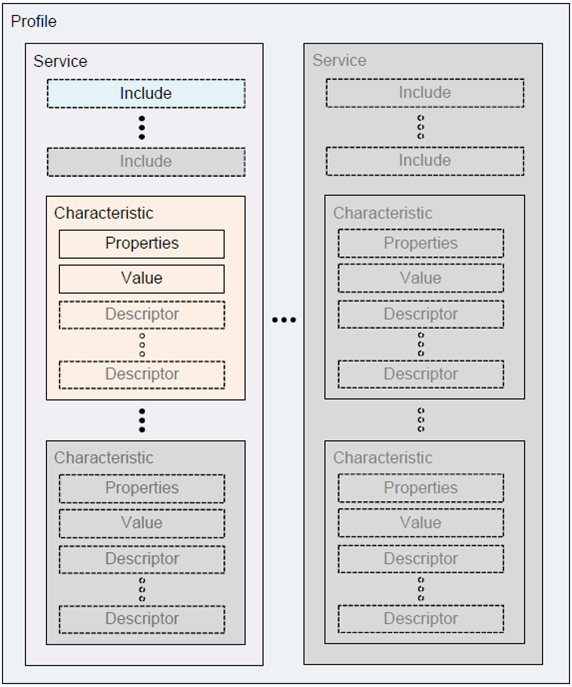
\includegraphics[width=0.6\textwidth,center]{fig/gatt}
\caption{Hierarki for GATT-profiler} %\todo{Kilde? \url{https://www.bluetooth.com/specifications/generic-attributes-overview}}
\label{fig:gatt}
\end{figure}

\subsubsection{Sikkerhet i BLE}
De største sikkerhetsproblemene til BLE generelt er passiv tyvlytting, \gls{mitm} og identitetssporing.
Bluetooth 4.0 ble annonsert i 2010, og er nå delvis utdatert når det gjelder sikkerhet. Alle paringsmetodene
til 4.0 og 4.1 kalles for \textit{LE Legacy Pairing}. 

For å unngå passiv tyvlytting, krypterer BLE dataen som sendes mellom to enheter med en sikker blokkchiffer (AES-CCM). Problemet oppstår
i nøkkelutvekslingen mellom de to enhetene. I den vanligste paringsmetoden i \textit{LE Legacy Pairing}, \textit{Just Works\texttrademark},
brukes en svak midlertidig nøkkel (nøkkelen er tallet 0). Dermed er det enkelt for en angriper å finne ut hva korttidsnøkkelen
blir med rå datakraft og gjetting. Andre paringsmetoder eksisterer, men disse trenger brukerinteraksjon eller andre trådløse protokoller (NFC).
De er imidlertid rimelig sikre mot \gls{mitm}.
%\todo{kilde: \url{https://eewiki.net/display/Wireless/A+Basic+Introduction+to+BLE+Security}}

4.2 introduserer \textit{LE Secure Connections}. I denne utgaven av Just Works\texttrademark-paring blir det kun generert
én langtidsnøkkel ved hjelp av Elliptic Curve Diffie Hellman asymmetrisk kryptering. Dette løser problemet med passiv
tyvlytting, men forbindelsen er fortsatt sårbar for \gls{mitm} siden autentisering mangler. Et lite tillegg til Just Works\texttrademark
der man sammenligner om to verdier er like gjør denne metoden sikker mot \gls{mitm}.

Etter at enhetene er paret, er det mulig å lagre nøklene på hver enhet slik at de kan gjenbrukes uten å gå igjennom hele
paringsprosessen på nytt. Dette kalles \textit{bonding}.

Bluetooth 5 som begynner å komme i produkter våren 2017, lover lengre rekkevidde og økt hastighet.

%https://electronics.stackexchange.com/questions/284056/can-ble-transactions-be-encrypted-without-pairing
%https://security.stackexchange.com/questions/100554/is-bluetooth-4-0-traffic-encrypted-by-default-design
%https://piratecomm.wordpress.com/2014/01/19/ble-pairing-vs-bonding/
%https://community.nxp.com/thread/332191

\subsection{Seriell kommunikasjon og GPIO}
Det er flere ulike kommunikasjonsprotokoller for å snakke med annen elektronikk og andre integrerte kretser.
Seriell kommunikasjon består, i sin enkleste form, av å sende og motta binærdata over en asynkron seriell datalink.
Figur \ref{fig:serial} viser oppsettet mellom to enheter. En seriell enhet må ha en port for å motta data (RX)
og en port for å sende data (TX).

\Gls{gpio} er et generisk tilkoblingspunkt på en datamaskin eller integrert krets. Det er et grensesnitt mellom enheten
og omverdenen som gjør det mulig koble til for eksempel knapper og lys. Tilkoblingspunktene kan være konfigurert som
input eller output. I output-modus kan tilstanden til et punkt være enten høy (typisk 5V eller 3.3V) eller lav (0V).
I input-modus leses også signalet som høyt eller lavt med en trekk opp- eller trekk ned-motstand, og kan dermed
brukes til \textit{interrupts}.
%\todo{Kilde: \url{https://www.raspberrypi.org/documentation/usage/gpio/}}

\begin{figure}
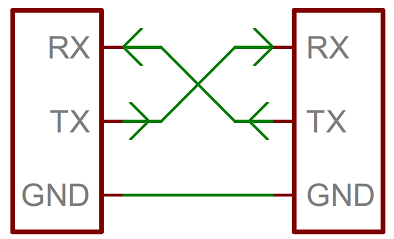
\includegraphics[width=0.5\textwidth,center]{fig/serial}
\caption{Seriell databuss}
\label{fig:serial}
\end{figure}

\section{Skyteknologi}
\blindtext

\subsection{Skybasert tingenes internett}
% \todo{Sikkerhet, personvern, kvalitetsattributter}
\blindtext

\subsection{AWS IoT}
\label{sec:aws_iot}
Amazon sin \gls{iot}-løsning i skyen (\gls{aws} \gls{iot}) ble annonsert 9. oktober 2015.
Viktige aspekter av denne løsningen er \textit{AWS IoT Device SDKs} som tilkobler mot 
en \textit{device gateway}, og en \textit{rules engine} som tillater løsningen å integrere
mot andre AWS-tjenester. Se figur \ref{fig:awsiot_how} for arkitekturoversikt.
Denne arkitekturen likner veldig på den \citet{iot_harvard_smart} foreslo i kapittel \ref{ch:background}.

\textit{Thing registry} er en liste av alle enheter tilkoblet tjenesten, og en \textit{device shadow}
holder styr på tilstanden til en enhet som kan hentes eller modifiseres fra andre applikasjoner.

\begin{figure}
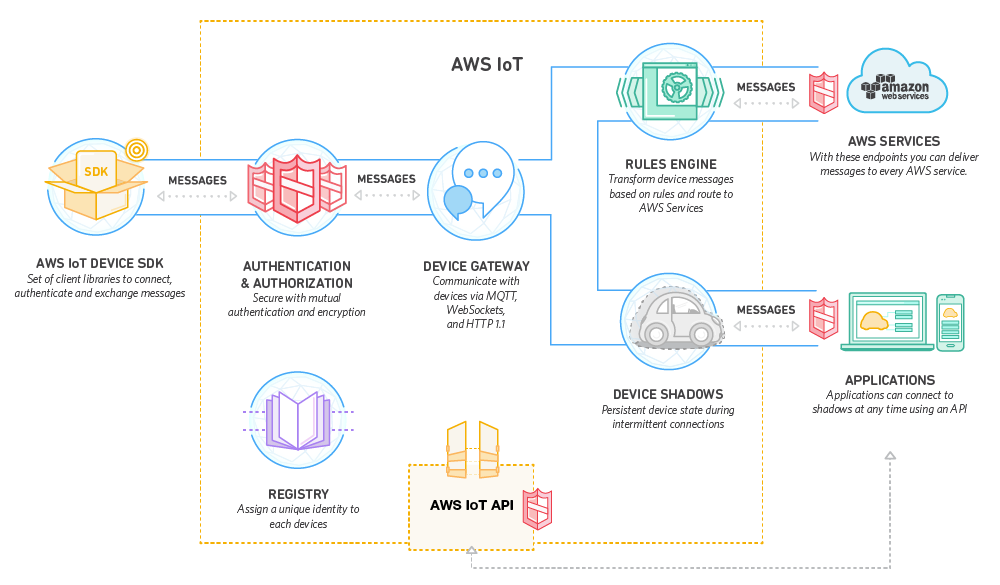
\includegraphics[width=1.0\textwidth,center]{fig/awsiot_how}
\caption{AWS IoT: Hvordan det virker \citep{aws_works}}
\label{fig:awsiot_how}
\end{figure}

\subsubsection{AWS IoT Device SDKs}
SDK-er er åpen kildekode på Github, og er tilgjengelige for embedded C, JavaScript (Node.js og nettleser),
Arduino Yún, Java, Python, iOS og Android \citep{aws_sdks}.

\subsubsection{Sikkerhet: Autentisering og tilgangskontroll}
AWS IoT tilbyr ende-til-ende-kryptering og gjensidig autentisering av alle meldinger med
\gls{tls} og klientside-X.509-sertifikater. Andre autentiseringsmetoder som Amazon sin egen SigV4-protokoll
er tilgjengelig også.

\subsubsection{Device gateway}
Device gateway fungerer som en skalerbar \textit{meldingsbroker} basert på publish-subscribe-mønsteret,
med støtte for MQTT (publish/subscribe), MQTT over WebSockets (publish/subscribe) og HTTP (publish).

\subsubsection{Rules engine}
Rules engine evaluerer innkommende meldinger etter at de passerer igjennom device gateway,
og videresender disse meldingene til resten av AWS-økosystemet avhengig av hvilke regler som er satt opp.
Dette betyr at meldinger for eksempel kan bli endret og sendt videre, lagret i en database, aggregert i en
dataanalyseløsning og brakt videre til andre skytjenester. \citet{aws_works} nevner AWS Lambda, Amazon Kinesis,
Amazon S3, Amazon Machine Learning, Amazon DynamoDB, Amazon CloudWatch og Amazon Elasticsearch Service som mulige
integrasjoner.

\subsubsection{Device shadows}
Alle enheter koblet til device gateway har en thing shadow som er et JSON-dokument
med nåværende tilstand og informasjon om enheten. En thing shadow til en ting er alltid tilgjengelig,
selv om enheten er koblet fra Internett. Den kan alltid bli hentet og endret over HTTP eller MQTT. En thing shadow
er identifisert med sitt unike navn. AWS IoT reserverer emnenavnene \textit{get}, \textit{update}
og \textit{delete} for å kommunisere med device shadows.

\subsubsection{Thing registry}
Et thing registry er en JSON-liste av alle tingene som er tilkoblet til tjenesten. Hver ting
har et navn, og kan valgfritt ha attributter i nøkkel-verdi-par, for eksempel modellnavn og watt
for en lyspære. Det er mulig å lage forskjellige typer ting og assosierere disse typene med en ting.

\subsection{Microsoft Azure IoT Hub}
Microsoft Azure IoT Hub har mange av de samme egenskapene som AWS IoT med andre navn: \textit{cloud gateway},
\textit{device twins} og \textit{identity registry}. Autentisering gjøres enten med et unikt token per enhet eller med
X.509-sertifikater. I praksis tilbyr de to skyteknologileverandørene akkurat det samme.

\begin{figure}
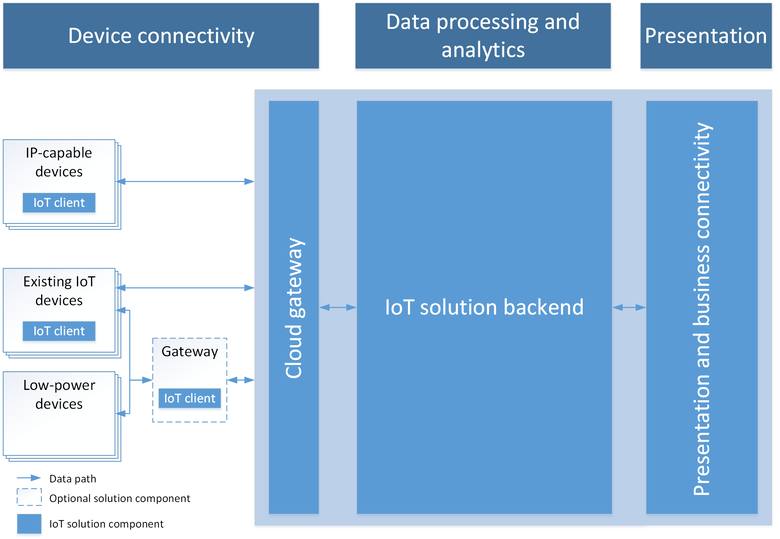
\includegraphics[width=1.0\textwidth,center]{fig/iot-reference-architecture}
\caption{Microsoft Azure IoT Hub: Løsningsarkitektur} % \todo{sitering?}
\label{fig:azure_iot}
\end{figure}

% \section{Utviklingsmiljø} \todo{Skal dette være med egentlig? Er det relevant å bable om Node.js her?}

\section{Prototypeplattform: Raspberry Pi Zero W}
Raspberry Pi Zero W er en liten og billig datamaskin med lavt strømforbruk lansert i februar 2017 (figur \ref{fig:pizero}).
Den har følgende spesifikasjoner: % \todo{https://www.raspberrypi.org/help/faqs https://www.raspberrypi.org/products/pi-zero-w/}
\begin{itemize}
    \item 1GHz, énkjerne-CPU
    \item 512MB RAM
    \item 802.11 b/g/n trådløs LAN
    \item Bluetooth 4.1 (BLE)
    \item Mini HDMI og USB On-The-Go-porter
    \item Micro SD-kortmodul
    \item HAT-kompatibel 40-pin header
    \item \textbf{Strømforbruk:} typisk 100mA i hvilemodus og maks 350mA under stress
    \item \textbf{Størrelse}: 65 mm × 30 mm × 5 mm
\end{itemize}

Figur \ref{fig:pizero_gpio} viser de ulike portene til \gls{gpio}-headeren. Det er flere kontakter for
jording, 5V, 3V, og noen porter kan brukes til seriell kommunikasjon og I2C i tillegg til \gls{gpio}.
Raspberry Pi Zero W kjører på Raspbian, et Debian-basert operativsystem laget spesielt for de ulike utgavene av
Raspberry Pi med Linux-kjernen i bunn..

\begin{figure}
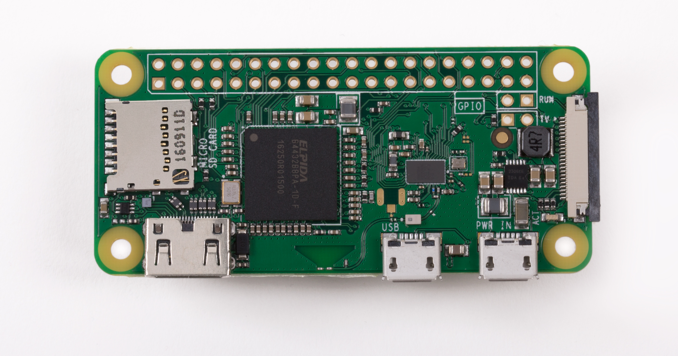
\includegraphics[width=0.8\textwidth,center]{fig/pizero}
\caption{Raspberry Pi Zero W. Foto: \url{https://www.raspberrypi.org}}
\label{fig:pizero}
\end{figure}

\begin{figure}
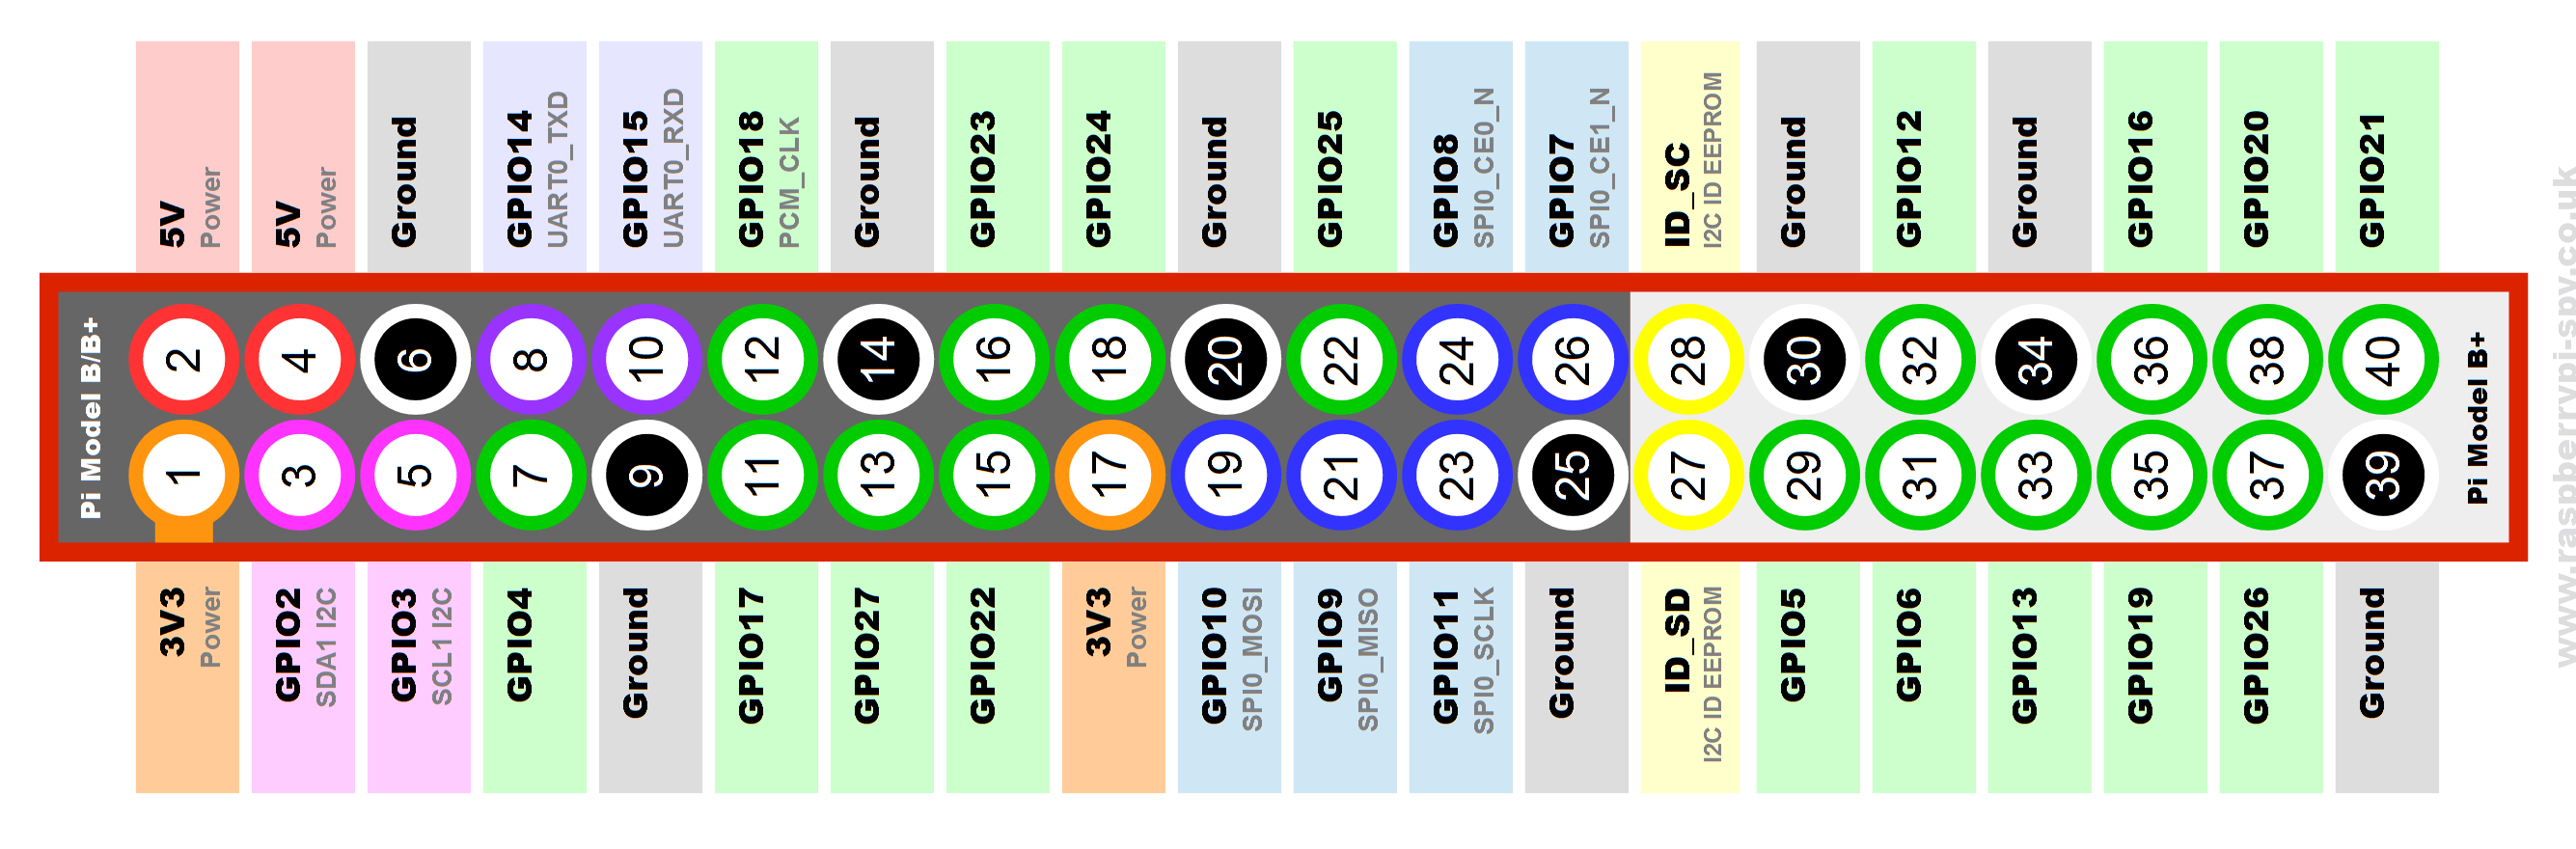
\includegraphics[width=1.0\textwidth,center]{fig/pizero_gpio}
\caption{Pi Zero W: GPIO header. Foto: \url{http://www.raspberrypi-spy.co.uk}}
\label{fig:pizero_gpio}
\end{figure}

\section{Sensorer og aktuatorer}
En sensor er en innretning som gir signal om en tilstand i den fysiske omverdenen. Eksempler
på sensorer kan være temperaturmåler, bevegelsessensor, ultralyd og trykknapp. Aktuatorer er innretninger som påvirker
den fysiske omverdenen på en eller annen måte, for eksempel lysdioder, buzzere og LCD-skjermer.
% https://www.ntnu.no/wiki/display/plab/1.+Generelt+om+aktuatorer+og+LED
% https://www.ntnu.no/wiki/display/plab/1.+Generelt+om+sensorer+og+trykknapper

\subsection{Pulsoksimeter}
Et pulsoksimeter er en sensor som måler oksygenmetning i blodet og pulsfrekvens.

Trondheim kommune låner ut en Nonin 3230 (se figur \ref{fig:nonin-3230}) til bruk i denne masteroppgaven.
Nonin 3230 er et pulsoksimeter med støtte for \gls{ble} 4.0. Dette pulsoksimeteret ble anbefalt av \citet{austad2016sensorer}
i rapporten \textit{Sensorer til støtte for avstandsoppfølging}. De trakk fram at alle Nonins produkter
er klinisk validerte, at det er støtte for \gls{ble}, % @TODO OG BLABLA NOE MER 

Nonin 3230 måler oksygenmetning fra 0 til 100\% og pulsfrekvens fra 18 til 321 slag per minutt. Den går på to
AAA-batterier, og er spesifisert for 2200 spotmålinger (25 sekunder per måling).

\begin{figure}
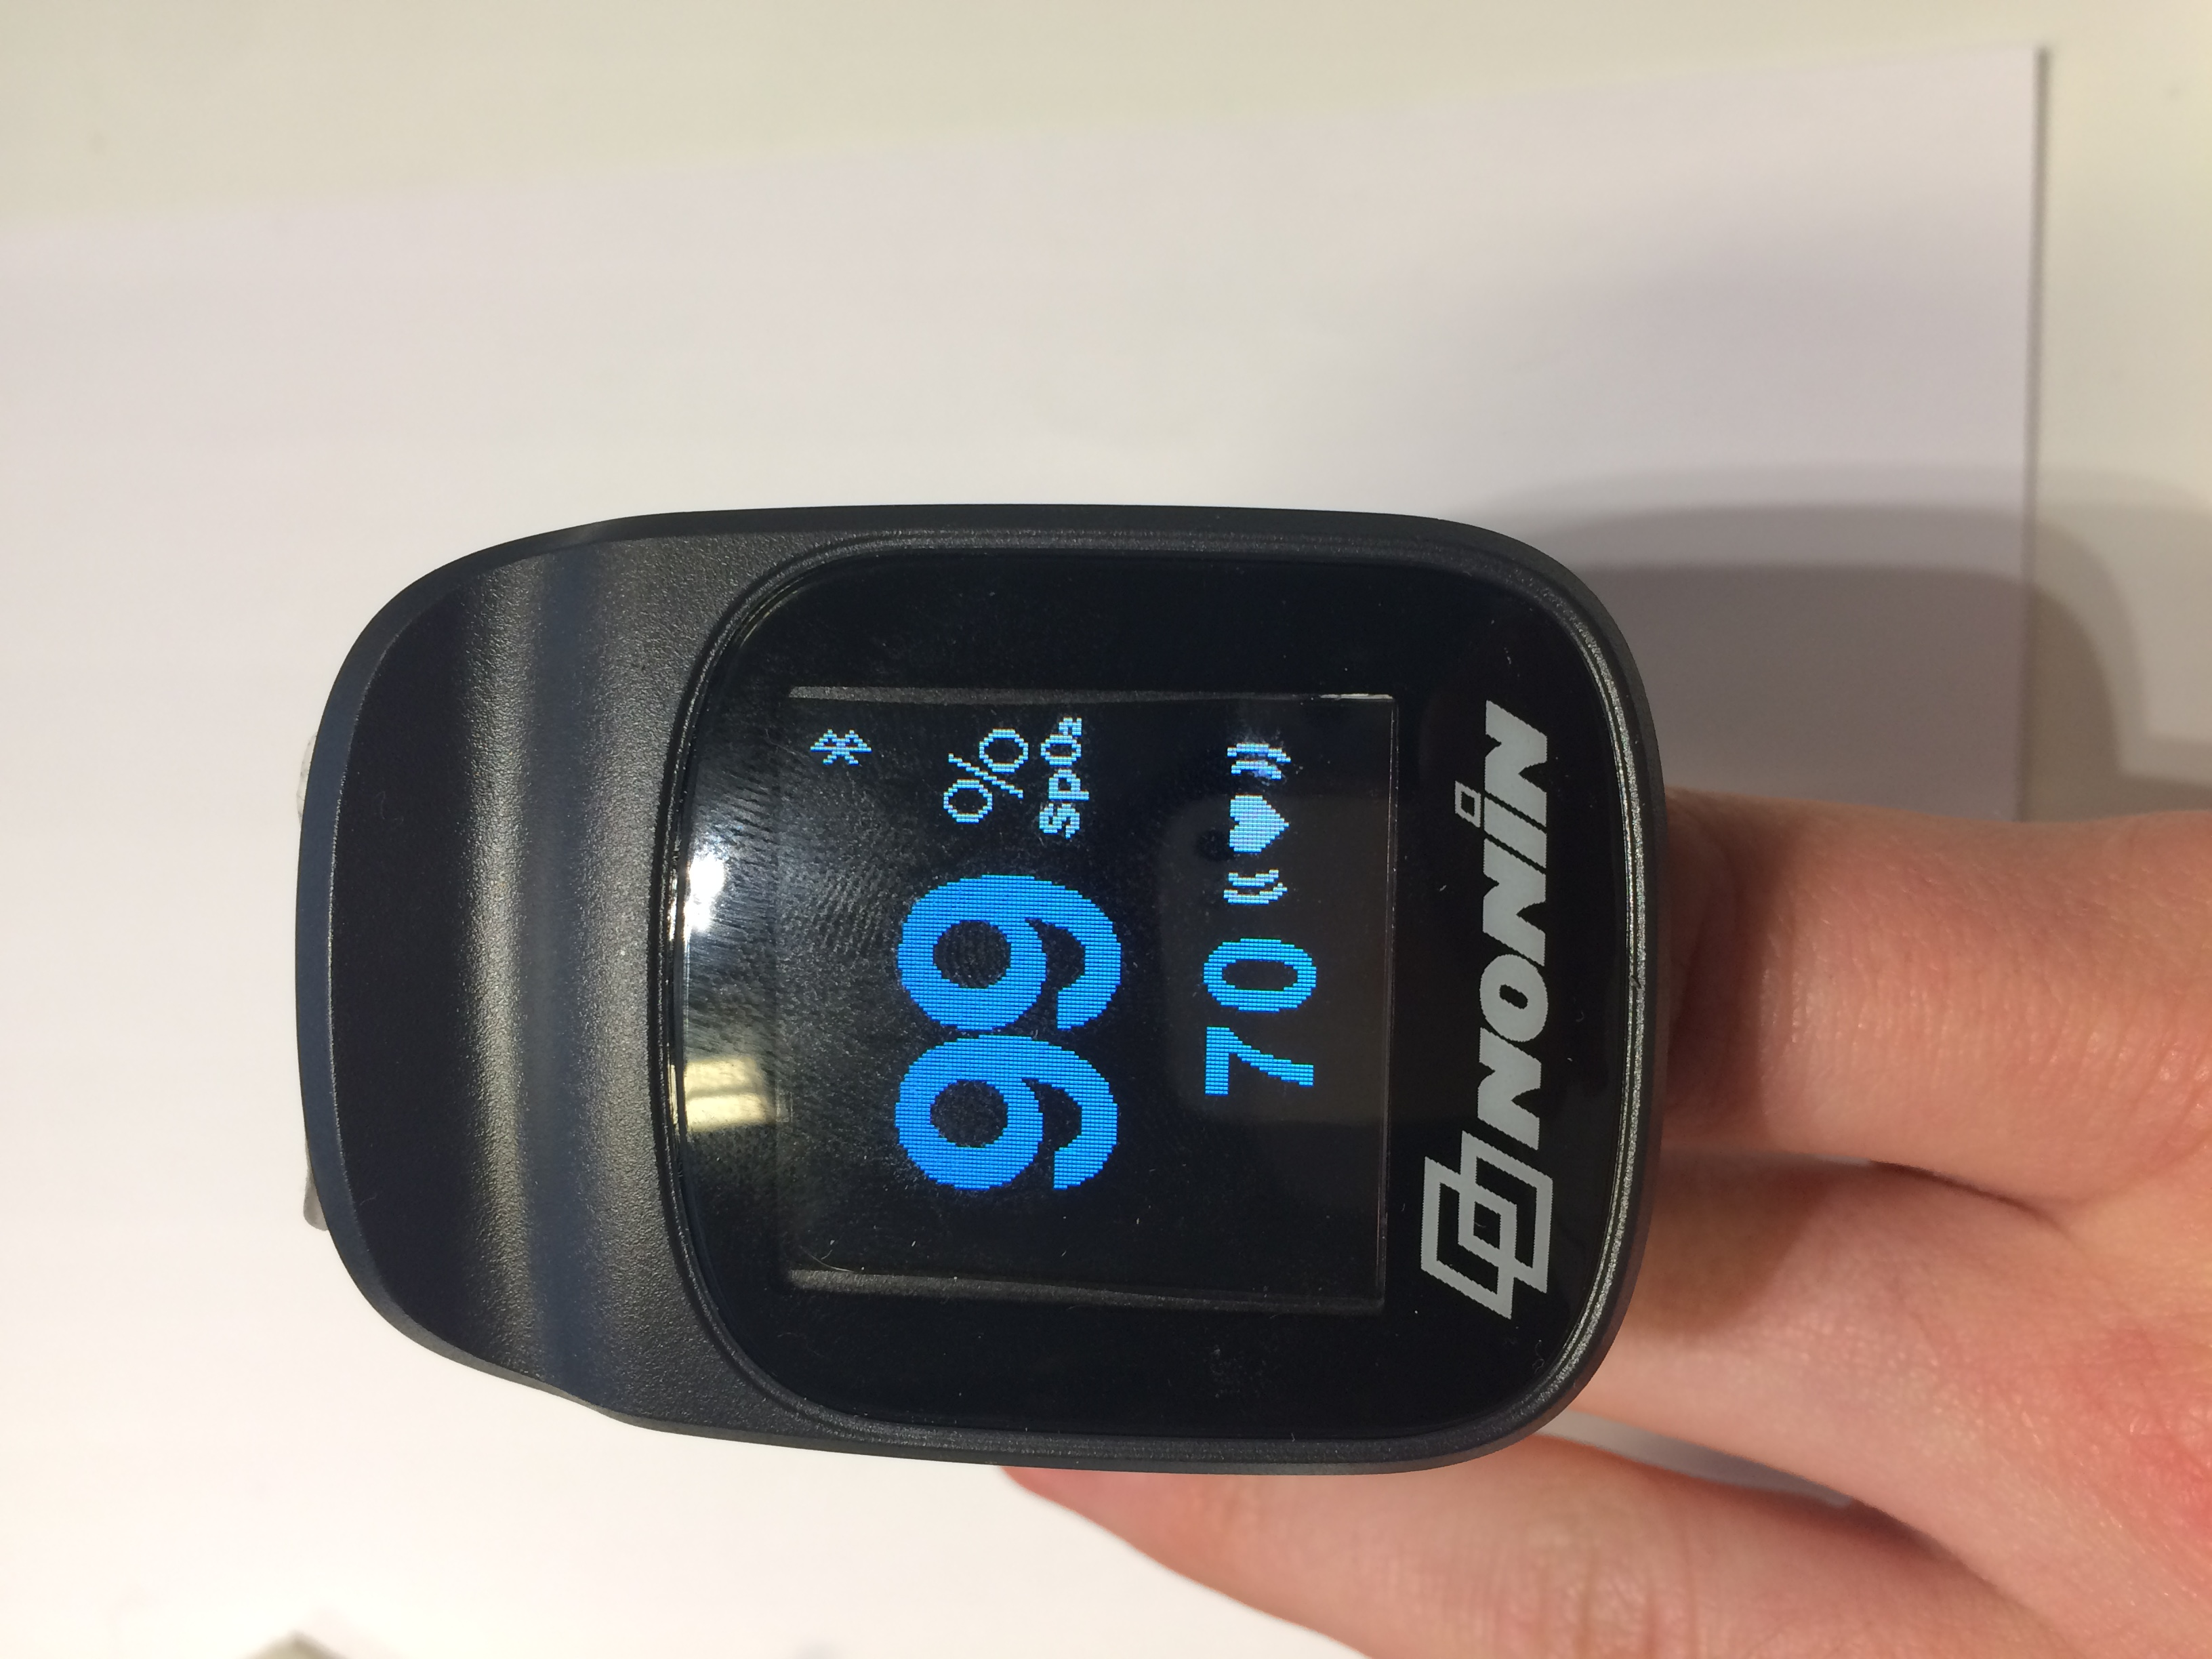
\includegraphics[width=0.75\textwidth, center]{fig/prototype/nonin3230ble}
\caption{Nonin 3230}
\label{fig:nonin-3230}
\end{figure}

%https://www.protocentral.com/sensors/1030-protocentral-pulse-oximeter-heart-rate-sensor-based-on-max30100.html
\subsection{Fingeravtrykksensor}
\subsection{Trykknapp}
\subsection{RGB LED}

\chapter{Design og implementasjon av et skytilkoblet pulsoksimeter}
\label{ch:implementation1}

Kapittelet beskriver hvordan en prototype av et skytilkoblet pulsoksimeter med innebygget autentisering ble utviklet.
Første del av kapittelet handler om valg av teknologien før blabla

\section{Valg av komponenter}
Løsningen består av følgende komponenter:

\begin{itemize}
  \item Raspberry Pi Zero W
  \item GT-511C3 (fingeravtrykksensor)
  \item Nonin 3230 (pulsoksimeter med \gls{ble})
  \item Standard trykknapp
  \item Tre RGB-lysdioder og én hvit lysdiode
  \item 3D-printet hus
\end{itemize}

Komponentene er presentert i forrige kapittel. Raspberry Pi Zero W ble valgt som prototypeplattform istedenfor
alternativer som Tessel 2 og Arduino Yún. Det var et ønske om å bruke JavaScript og Node.js som utviklingsmiljø, og Arduino
bruker C/C++ som utviklingsspråk. Tessel 2 er en prototypeplattform basert på Node.js, men har få konfigurasjonsmuligheter
og \gls{ble} er ikke innebygget.

\section{Oversikt over løsning}


\begin{figure}
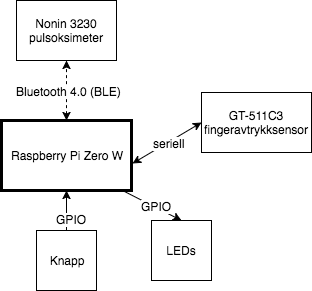
\includegraphics[width=0.55\textwidth, center]{fig/prototype/oversiktlosning}
\caption{Sammenhengen mellom de ulike komponentene}
\label{fig:prototypeoversikt}
\end{figure}

\section{Komponenter}

\subsection{Trykknapp og lysdioder}

\begin{figure}
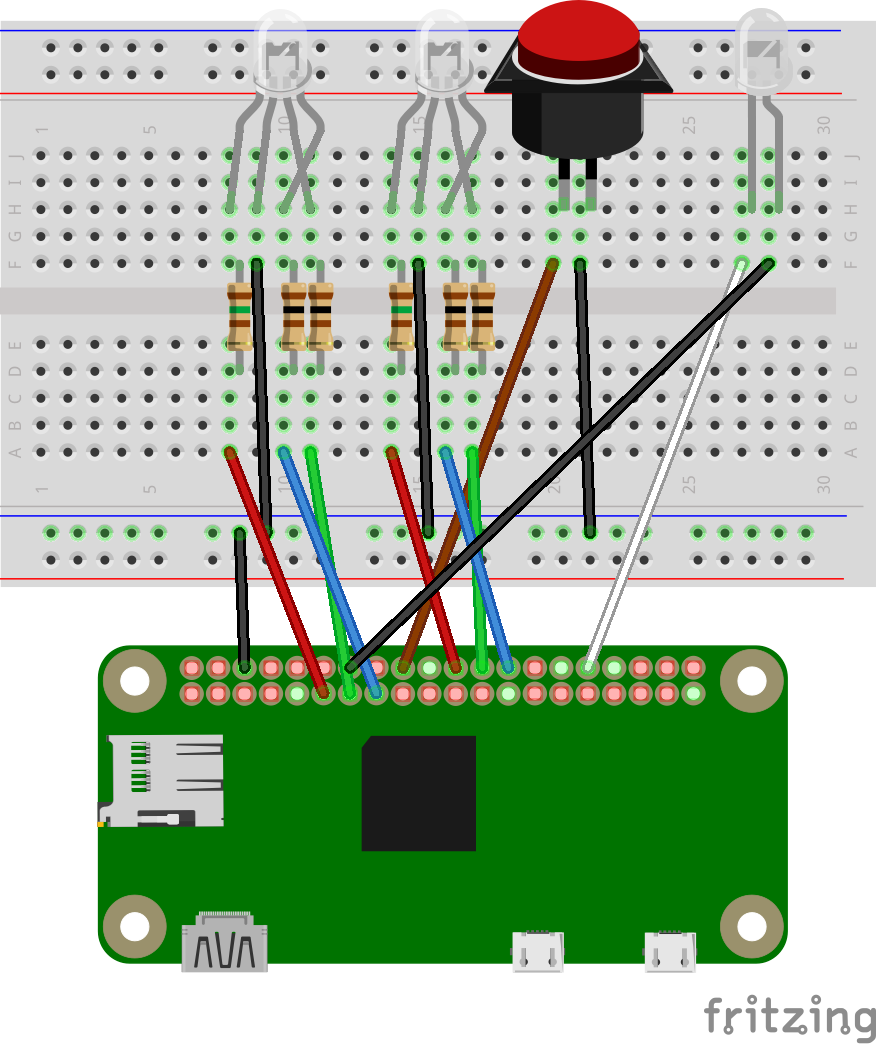
\includegraphics[width=0.75\textwidth, center]{fig/prototype/breadbord}
\caption{Oppkobling av trykkknapp og lysdioder}
\label{fig:breadboard}
\end{figure}

\begin{figure}
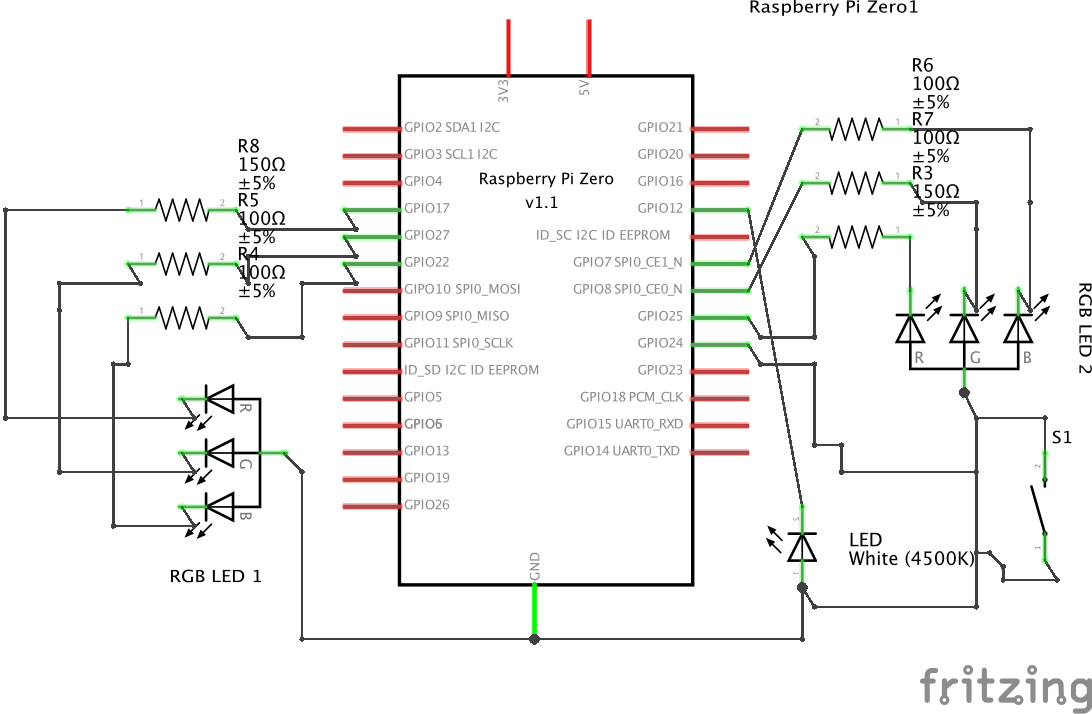
\includegraphics[width=0.95\textwidth, center]{fig/prototype/schmeatic}
\caption{Koplingsskjema av trykknapp og lysdioder}
\label{fig:schematics}
\end{figure}

\subsection{GT-511C3}

\subsection{Nonin 3230}
Trondheim kommune lånte ut en Nonin 3230 (se figur \ref{fig:nonin-3230}) til bruk i denne masteroppgaven.
Nonin 3230 er et pulsoksimeter med støtte for \gls{ble} 4.0. Dette pulsoksimeteret ble anbefalt av \citet{austad2016sensorer}
i rapporten «Sensorer til støtte for avstandsoppfølging». De trakk fram at alle Nonins produkter
er klinisk validerte, støtten for Bluetooth Smart,   

Utgaven Trondheim kommune har kjøpt inn bruker en proprietær Bluetooth-tjeneste med 128 bit \gls{uuid}.
I nyere utgaver kan man også bruke den åpne spesifikasjonen til «Bluetooth SIG Pulse Oximeter Service».
Den proprietære tjenesten heter «Nonin Oximetry Service» og har \gls{uuid} \textit{46a970e00d5f11e28b5e0002a5d5c51b}.
Tjenesten har to karakteristikker -- «Nonin Oximetry Measurement» som sender data hvert sekund som spesifiert
i tabell \ref{table:nonin-datapacket} og «Nonin Control Point» som kan brukes til å synkronisere skjermen,
indikere at en måling er ferdig, eller sette sikkerhetsmodus. 

Et \gls{npm}-biblotek (fotnote url) kalt \textit{nonin-3230-ble} ble utviklet for å gjøre integrasjonen mot sensoren enklere.
Biblioteket baserer seg på \textit{noble-device} (fotnote), og inneholder metoder for å oppdage et pulsoksimeter,
koble til, lytte etter ny sensordata og indikere at en måling er ferdig. Sensordata kommer som et JavaScript-objekt
og inneholder teller, pulsfrekvens, SpO2 og et statusobjekt (tabell \ref{table:nonin-status}).
Koden er lagt ved i appendiks \ref{lst:nonin-3230-library}.
Eksempel på bruk kan finnes i kodesnutt \ref{lst:nonin-3230-usage}.

\begin{figure}
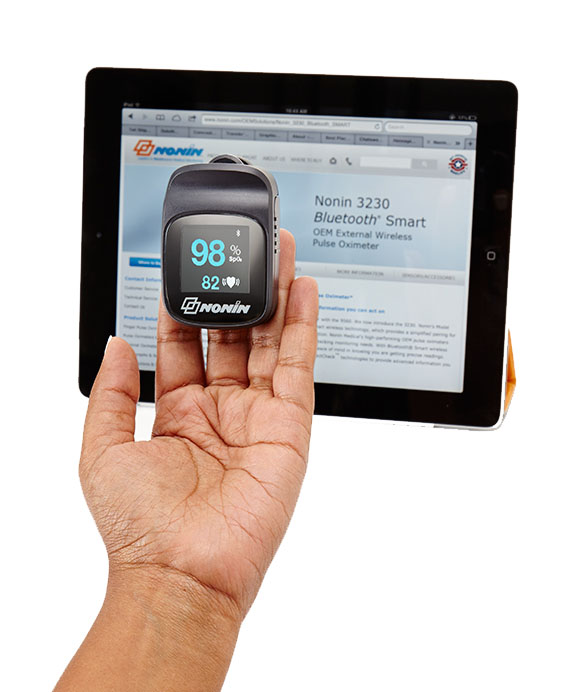
\includegraphics[width=0.95\textwidth, center]{fig/Nonin3230iPad}
\caption{Nonin 3230. Foto: Nonin}
\label{fig:nonin-3230}
\end{figure}

\begin{minipage}{\linewidth}
\begin{lstlisting}[frame=single, language=JavaScript,
    caption=Bruk av nonin-3230-ble, label=lst:nonin-3230-usage]
const Nonin3230 = require('nonin-3230-ble');

Nonin3230.discover((pulseOximeter) => {
  pulseOximeter.connectAndSetup((error) => {
    if (error) {
      console.error(error);
    }
    let counter = 0;
    // receive a new measurement every second
    pulseOximeter.on('data', (data) => {
      // data: { counter: int, pulseRate: int, oxygenSaturation: int, status: object }
      counter++;
      if (counter > 15) {
        pulseOximeter.stopMeasurement(() => console.log('Stopped'));
      }
    });
  });
});
\end{lstlisting}
\end{minipage}

Kildekoden er åpen og kan kjøres fra alle enheter som har støtte for Node og \gls{ble}.


\begin{table}[]
\centering
\begin{tabular}{|l|l|l}
\hline
\multicolumn{3}{|l|}{\textbf{Datapakke til oksimeter}} \\ \hline
\textbf{Byte} & \textbf{Felt} & \multicolumn{1}{l|}{\textbf{Beskrivelse}} \\ \hline
1 & Lengde & Antallet bytes inkludert denne. \\ \hline
2 & Status & \multicolumn{1}{l|}{Indikerer nåværende enhetsstatus (tabell \ref{table:nonin-status}).} \\ \hline
3 & Batterispenning & \multicolumn{1}{l|}{Spenningsnivået til batteriene som brukes.} \\ \hline
4-5 & \begin{tabular}[c]{@{}l@{}}Perfusjonsindeks\\ (PI)\end{tabular} & \multicolumn{1}{l|}{PI = AC/DC*100\%} \\ \hline
6-7 & Teller & \multicolumn{1}{l|}{\begin{tabular}[c]{@{}l@{}}Verdien økes hvert sekund (0-65535). Kan bli brukt\\ til å sjekke at det ikke er noe datatap.\end{tabular}} \\ \hline
8 & SpO2 & \multicolumn{1}{l|}{SpO2-prosent, 0-100 (gjennomsnitt av fire slag).} \\ \hline
9-10 & Pulsfrekvens & \multicolumn{1}{l|}{\begin{tabular}[c]{@{}l@{}}Pulsfrekvens i slag per minutt, 0-321\\ (gjennomsnitt av fire slag).\end{tabular}} \\ \hline
\textgreater11 & Reservert & \multicolumn{1}{l|}{Reservert til fremtidig bruk} \\ \hline
\end{tabular}
\caption{Nonin 3230: Format på datapakke ref: nonin integration guide}
\label{table:nonin-datapacket}
\end{table}

\begin{table}[]
\centering
\begin{tabular}{|l|l|l}
\hline
\multicolumn{3}{|l|}{\textbf{Statusfelt (aktiv høy)}} \\ \hline
\textbf{Bit} & \textbf{Felt} & \multicolumn{1}{l|}{\textbf{Beskrivelse}} \\ \hline
7 & Reservert & Reservert til fremtidig bruk. \\ \hline
6 & Kryptering & \multicolumn{1}{l|}{\begin{tabular}[c]{@{}l@{}}1 = tilkoblingen er kryptert\\ 2 = tilkoblingen er ikke kryptert\end{tabular}} \\ \hline
5 & Lavt batteri & \multicolumn{1}{l|}{Batterinivået er lavt. Bytt batteri.} \\ \hline
4 & CorrectCheck & \multicolumn{1}{l|}{\begin{tabular}[c]{@{}l@{}}1 = OK\\ 2 = Plasser fingeren lengre inn i enheten\end{tabular}} \\ \hline
3 & Søker & \multicolumn{1}{l|}{Oksimeteret søker etter etterfølgende pulssignaler.} \\ \hline
2 & SmartPoint & \multicolumn{1}{l|}{\begin{tabular}[c]{@{}l@{}}Brukt til å indikere at dataen har bestått SmartPoint-\\ algoritmen.\end{tabular}} \\ \hline
1 & Lavt/svakt signal & \multicolumn{1}{l|}{\begin{tabular}[c]{@{}l@{}}Styrken til pulssignalet er 0,3 \% modulasjonsgrad\\ eller mindre.\end{tabular}} \\ \hline
0 & \begin{tabular}[c]{@{}l@{}}Indikering av\\ skjermsynkronisering\end{tabular} & \multicolumn{1}{l|}{\begin{tabular}[c]{@{}l@{}}Indikerer at skjermen er synkronisert med\\ innsamleren av data.\end{tabular}} \\ \hline
\end{tabular}
\caption{Nonin 3230: Format på statusfeltet til datapakke ref: nonin integration guide}
\label{table:nonin-status}
\end{table}


\section{Serversideløsning}
\subsection{AWS IoT}
\subsection{AWS Lambda}
\subsection{InfluxDB og Grafana}

\subsection{Begrensninger med løsningen}
\chapter{Evaluering av pulsoksimeter}
\label{ch:evaluation1}

\section{Fokusgruppe med Trondheim kommune}
\section{Fokusgruppe med SINTEF}
\chapter{Diskusjon}
\label{ch:discussion}

\section{Utfordringer for teknologi i avstandsoppfølging}
Kapittel \ref{ch:case} viser at Trondheim kommune ønsker å være tidlig ute med ny teknologi, men at dette kan være vanskelig å
få til i praksis. De er også klare på at det er teknologien som skal understøtte tjenesten og ikke motsatt. Den største
utfordringen er å få rullet ut tjenesten til flere hundre brukere i en stor organisasjon. Det er i denne konteksten
man må se hvordan teknologi kan hjelpe kommunen med å løse sine problemer. Kommunen opplever at brukerne er veldig forskjellige, og
at de har forskjellige behov. Det er ikke alle som kan bruke sensorer. De er klare på at tjenesten må tilpasses individuelt til hver
enkelt bruker. Målet er at brukeren skal oppleve økt trygghet.

Under evalueringen pekte kommunen på at de i dag har for dårlige verktøy
til å se på måledata, og dermed ikke kan nyttiggjøre seg sensorteknologien så veldig godt. Dette er noe som kommunen og andre kan jobbe med
for å forbedre. Det er ikke så komplisert å sette opp enkle grafsystemer. Grafana som ble brukt under dette prosjektet er åpen kildekode.
Kommunen har ikke så mye annet valg enn å forholde seg til leverandører av programvare og helseprodukter dersom de
ikke skal ha utviklere ansatt hos seg. Leverandørene og produsentene
har dermed et stort anvar for å lage gode løsninger og ta i bruk ny teknologi tidlig. Det er tydelig at de løsningene kommunen bruker i dag
ikke ser så moderne ut og bruker modifisert hyllevare. Allikevel sier brukerne at de synes systemene er greie å bruke. Nonin kunne ha laget
et mer helintegrert pulsoksymeter, men det ville komplisert deres ansvarsområder veldig. Det er enklere for produsenten å konsentrere seg om
selve oksimeterteknologien og gi et grensesnitt for andre å integrere med.

\section{Utvikling og evaluering av en frittstående prototype}
Utviklingen av prototypen skjedde ikke så brukernært som det kanskje var ønsket i starten av prosjektet. Det ble kun tid
til én iterasjon der målet først var å få til to runder med tilbakemelding i mellom. Det tok litt tid før alle komponenter kom fram,
og i starten ble en annen prototypeplattform valgt og prøvd istedenfor Raspberry Pi Zero W.
Det var også opprinnelig et ønske om å få til mer toveiskommunikasjon, for eksempel et varsel med pulserende lys til brukeren
når det var tid for å foreta en måling. Dette ble det ikke tid til, men kan være noe å prøve ut i fremtiden. I implementasjonsperioden
var det utfordrende å få klientprototypen til å fungere tilfredsstillende siden det var så mange komponenter som skulle fungere sammen
med forskjellige eventer, avbrudd og en komplisert tilstandsmaskin. Disse utfordringene gjorde at det ikke ble så god tid til å jobbe
med toveiskommunikasjon og en større skyimplementasjon.

Fingeravtrykket fra enheten må lagres i skyløsningen som en fil, og knyttes til hver enkelt bruker. Når brukeren
ønsker å autentisere seg, må fingeravtrykket hentes til enheten, og så sjekkes. Tofaktorautentisering er at man
sier hvem man er på to forskjellige måter. Som oftest er det to av følgende: noe en vet, noe en har eller noe en er.
Enhet med sertifikat er noe en har, og fingeravtrykk er noe en er. I teorien kan det dermed bety at prototypen
oppfyller kravene til en tofaktorautentisering, men dette er noe som må undersøkes nærmere med eksperter på sikkerhet.

Fordelen med å basere seg på eksisterende plattformer som Android og iOS er at man får mye gratis i form
av blant annet sikkerhetsoppdateringer og rammeverk for brukergrensesnitt. Dette er noe en må ordne selv i en
frittstående løsning. Eksisterende plattformer har allerede mye infrastruktur som kan av laste kommunen. I tillegg
har mange av brukerne enheter som kjører på disse plattformene fra før av. iOS-telefoner og mange Android-telefoner
har innebygget fingeravtrykkssensor og muligheten til å styre disse fra programvare. Det kunne erstattet behovet for
en tredjepartssensor. Det ville muligens tatt kortere tid å implementere noe på disse plattformene siden det ville vært
mindre behov for å skrive helt nye integrasjoner mot komponenter og mindre jobb med den fysiske utformingen.

\section{En arkitektur for skybasert IoT}
En arkitektur for skybasert IoT for avstandsoppfølging kan være basert på AWS IoT som gir mye verdi for en utvikler ut av boksen.

MQTT ble brukt som kommunikasjonsprotokoll mellom prototype og skyløsning. Denne protokollen egner seg kanskje enda bedre for sensorer
som sender data kontinuerlig. Brukeren sender 20 sekunder med data hver dag i bruksscenarioet som ble skissert i dette prosjektet. Det er ikke så veldig
mye data. Den samme dataen kunne blitt sendt over HTTPS og en standard arkitektur som REST istedenfor. Det hadde vært mulig å bruke
en mer tradisjonell backendløsning istedenfor å basere seg på AWS IoT. Istedenfor sertifikater for autentisering
kunne en brukt tokens med så og så lang gyldighet som bevis på at enheten er logget inn. Spørsmålet er hvor mye verdi AWS IoT egentlig gir
for avstandsoppfølging.

Device shadows ble ikke brukt i dette prosjektet, men det kunne gitt en bra base for å håndtere tilstanden til hver enhet, og manipulere denne tilstanden
fra en adminapplikasjon. Det hadde vært relevant for å implementere en økt grad av toveiskommunikasjon. AWS gir flere slike nyttige verktøy for
å håndtere infrastrukturen på en enklere måte.
% noe om sanntidsanalyse

\section{Metodediskusjon}
Det hadde vært nyttig med mer teknisk informasjon om hvordan HelsaMi+ fungerer for å sammenligne,
se hvor langt de har kommet sikkerhetsmessig og hva de tenker om fremtiden. Leverandøren Imatis ble kontaktet for et
intervju, men svarte ikke på henvendelsen. Kanskje mer burde blitt gjort for å snakke med en leverandør av tekniske løsninger
til dette prosjektet. Det er en viktig komponent som mangler litt.

Hele temaet er også veldig stort, og det hadde kanskje vært
lurere å snevret inn hvilke kvalitetskrav man skulle sette ekstra søkelys på, og hvordan disse kravene
skulle vært testet slik at en kunne gjort et bedre dypdykk
og snakket med eksperter innenfor det området.

\section{Tillit til forskningen} % Dag: validitet (??)
\label{sec:validitet}

\subsection{Bekreftbarhet og pålitelighet}
Tidligere i kapittelet ble fremgangsmåten til studiet presentert. All kode ligger åpent tilgjengelig på Internett slik at hvem som helst kan
titte på den. Transkriberinger av intervjuene er tilgjengelige ved forespørsel. Tidligere ble implementasjonen av prototypen beskrevet i
så god detalj at det er mulig å lage noe tilsvarende kun ved å lese i teksten og se på koden.

\subsection{Troverdighet}
Alle intervjuene med Trondheim kommune må tolkes med det faktum at prosjektlederne har en tilknytning som
gjør at de ønsker at avstandsoppfølgingprosjektet
skal lykkes i bakhodet. Aktører direkte involvert i et prosjekt er mottakelige for bekreftelsestendenser der man søker etter å bekrefte noe
man allerede tror. Selv om SINTEF er en tredjepart som bistår Trondheim kommune, er de også mye involvert i prosjektet.
Det er mulig at forskningen kunne blitt enda mer troverdig med en kritisk tredjepart uten direkte tilknytning til velferdsteknologiprosjektet i Trondheim --
gjerne en stemme som ikke er udelt positiv til avstandsoppfølging som teknologi for velferd.
Fordelen med å snakke med personer som jobber med avstandsoppfølging i Trondheim kommune, er at de har veldig god kunnskap om temaet
og muligheten til å sammenligne løsningen som presenteres i denne forskningen med noe som eksisterer i praksis i dag.
De er en troverdig stemme i avstandsoppfølgingdebatten.

\subsection{Overførbarhet}
Spørsmålet som må stilles er om funnene og arbeidet gjort i dette prosjektet kan overføres til avstandsoppfølging som generelt tilfelle.
Trondheim kommune brukes som eksempel, og konklusjonen vil generalisere med kun dette tilfellet som bakgrunn.
Er det faktisk mulig å finne noen implikasjoner for utviklingen av skybasert \gls{iot} som teknologisk plattform for avstandsoppfølging?
Hvilke resonnementer og argumenter er i så fall disse resonnementene fundert i?
% @Todo ??? 
% Det som taler for at man kan det er at
% Det som taler mot er at 

\iffalse
\section{Begrensninger med
prototypen}\label{begrensninger-med-prototypen}

\begin{itemize}
\tightlist
\item
  Lav grad av toveiskommunikasjon implementert i prototypen, men rammeverket gjør det mulig.
\item
  Fingeravtrykk-template lagres direkte på sensoren, den burde blitt
  hentet fra sensoren og så lagret i skyen. Deretter burde den blitt
  hentet hver gang man trengte den.
\item
  Paring og bonding med Bluetooth. Enheten må pares hver gang i
  prototypen. Dette er en begrensning med det underliggende rammeverket
  som brukes.
\item
  I prototypen brukes MQTT over WebSockets til å sende data. Men det er
  såpass få målepunkter som sendes hver dag at man like gjerne kunne
  brukt HTTP REST med kryptering. Det er få fordeler med å bruke en
  protokoll som MQTT i dette prosjektet. Det hadde vært mer relevant om
  sensorene sendte data kontinuerlig hele døgnet.
\end{itemize}

\section{Sikkerhet}\label{sikkerhet}

\begin{itemize}
\tightlist
\item
  Tofaktorautentisering
\item
  Hva oppfyller kravene til tofaktorautentisering? Oppfyller
  klientsertifikat og enhet utplassert i hjem sammen med
  fingeravtrykksensor kravene?
\item
  Hvilke alternativer finnes det til å bruke fingeravtrykkssensor som
  autentisering? Både med tanke på brukbarhet og sikkerhet.
\item
  Bluetooth
\item
  BLE har flere sikkerhetsproblemer, spesielt i versjon 4.0 og 4.1. Skal
  man gjøre en oppfordring om kun å bruke Bluetooth 4.2? Hvilke
  avveininger og anbefalinger burde man gjøre dersom man må bruke en
  enhet med 4.0 eller 4.1? Det tar lang tid å ta i bruk en ny
  Bluetooth-standard. Produsenter av velferdsteknologi må følge med på
  den teknologiske utviklingen. Problemer her: tar lang tid å få et
  produkt godkjent, koster sikkert masse penger.
\end{itemize}

\section{Personvern og datalagring}\label{personvern-og-datalagring}

\begin{itemize}
\tightlist
\item
  Krav om at norske helsedata skal ligge i Norge. Dermed kan man ikke
  bruke en eksisterende skyløsning som AWS. AWS lagrer data i Europa.
  Det fører til at mye av infrastrukturen må lages fra bunnen av. Snakk
  om at Azure skal få til en løsning der man har hele økosystemet
  kjørende i Norge.
\item
  Ny personvernforordning gir flere rettigheter til forbrukere. Det
  gjelder blant annet kontroll på egen data, oversikt over hva den
  brukes til, mulighet til å slette den osv. Man må kunne argumentere
  for at dataen som lagres er nyttig for forbrukeren. Er da å lagre all
  sensordataen nyttig? Kan man argumentere for det?
\end{itemize}

\section{Frittstående løsninger kontra nettbrett, mobil,
PC}\label{frittstuxe5ende-luxf8sninger-kontra-nettbrett-mobil-pc}

Diskusjon og drøfting på bakgrunn av evalueringen om hvor vellykket det
var å implementere en frittstående løsning. Hvilke fordeler og ulemper
har man med å ta i bruk et eksisterende økosystem? Stikkord:
sikkerhetsoppdateringer, vedlikehold, innkjøpskostnad, hva har brukere
hjemme osv.

\section{Metodediskusjon}\label{metodediskusjon}

\begin{itemize}
\tightlist
\item
  Diskutere forskningsmetodene som er brukt? Hvor stor troverdighet kan
  man ha til forskningen? Kunne noe vært gjort annerledes?
\end{itemize}
\fi

\chapter{Konklusjon}
\label{ch:conclusion}

\section{Forskningsspørmål 1}
\textbf{\fs{1}}

I Trondheim kommune har ca. 70 brukere fått avstandsoppfølging hjemme. Det
foregår med et Android-nettbrett brukerne får utlevert. Dette nettbrettet har en
applikasjon der brukerne kan svare på hvordan dagsformen er. Spørsmålene er
tilpasset diagnosen til brukeren. I samråd med fastlegen har brukeren en
egenbehandlingsplan på papir som iverksettes på bakgrunn av helsetilstanden. Fastlegen
har ikke direkte tilgang til avstandsoppfølgingssystemet per i dag. Koordinasjon skjer via
helsevakta i Trondheim kommune. Seks brukere har fått sensorer (pulsoksymeter, vekt, blodtrykksmåler) de kan bruke
til målinger. Dette gjøres også via applikasjonen. Helsevakta får tilgang på
spotmålingen og svarene på spørsmålene i en adminapplikasjon.
Tilbakemeldingene på prosjektet i seg selv er veldig positive.

Prosjektledelsen har hatt utfordringer med stabiliteten til sensorløsningen.
De ser også utfordringer med personvern og å la brukeren få muligheten til å administrere og se mer av sin egen data.
Kommunen jobber med å få til sertifikater på nettbrettene, men det er ikke så lett. En annen erfaring
kommunen har gjort seg, er at brukerne er veldig forskjellige. Kommunen ønsker å være tidlig ute med
ny teknologi, men det viser seg å ikke være så enkelt å få til i praksis.

\section{Forskningsspørmål 2}
\textbf{\fs{2}}

En mulig arkitektur for realisering av skybasert \gls{iot} for
avstandsoppfølging er en klient-server-arkitektur basert på arbeidet som er
gjort i dette prosjektet med noen små modifikasjoner. Arkitekturen har en hub som
alle sensorene kobler seg på. Sensorene kommuniserer med huben med Bluetooth 4.2
eller nyere. Alle sensorer skal bondes med huben slik at sensorene ikke må pares
på nytt hver gang det skal sendes data. En mulig strategi for autentisering er å
bruke et klientsidesertifikat, og at dette sertifikatet er unikt for hver bruker
av løsningen. Dette er mest egnet for en backendløsning som håndterer
sertifikater, for eksempel AWS IoT, der MQTT over \gls{tls} med egne sertifikater
støttes. Det er helt klart mulig å benytte andre metoder for autentisering slik
at brukeren slipper å skrive inn passord hele tiden. Transport av data skal
uansett alltid skje med ende-til-ende-kryptering (\gls{tls}).

Arkitekturen har en regelbasert backend der dataen lagres fortløpende og
prosesseres i sanntid. Denne arkitekturen løser ikke problemer knyttet til personvern
og datalagring. Det er noe som må implementeres på toppen av skyløsningen. AWS gir allikevel
mange gode verktøy ut av boksen for å få til dette. Det kan understøtte mange av de
tjenesteutfordringene som HelsaMi+ opplever i dag.

\section{Forskningsspørmål 3}
\textbf{\fs{3}}

Prosjektledere i Trondheim kommune mente at prototypen hadde tilstrekkelig
brukskvalitet til å rulles ut til brukere. De mente imidlertid at det kanskje var bedre at
sensor og hub var adskilt og ikke koblet sammen til ett produkt. Prisen på prototypen
ble vurdert som rimelig. Indikering av at en måling er ferdig på skjermen til pulsoksymeteret
var noe kommunen ikke hadde med i sin løsning.

Forskere ved SINTEF var enige i at sensor og hub heller kunne vært adskilt, og trakk
fram at prototypen manglet muligheten til å svare på hvordan
dagsformen er. De så for seg at man kunne utvide prototypen med flere moduler,
for eksempel en modul med muligheten til å svare på spørsmål.

\section{Forskningsspørmål 4}
\textbf{\fs{4}}

Konklusjonen til dette forskningsspørsmålet deles opp
i avsnittene sikkerhet og autentisering, personvern, utviklingsomgivelser og
pris.

\subsection{Sikkerhet og autentisering}
\begin{itemize}
  \item Benytt ende-til-ende-kryptering (TLS).
  \item Autentiser brukeren med sertifikater eller tokens og benytt tofaktorautentisering.
  \item En moderne skytjeneste som AWS med sin løsning AWS IoT gir
      god innebygd sikkerhet som standard med TLS og sertifikater. Dette gjelder fra klient til skyen,
      men i en del tilfeller vil man ha et sikkerhetsproblem mellom klient og sensor.
  \item Bruk den nyeste utgaven av Bluetooth-standarden mellom klient og sensor som sensoren din
  støtter. Helst utgave 4.2 eller nyere. Hvis du må bruke en eldre versjon må
  du være observant på hvilke angrepspunkter som finnes og minimere risikoen for
  sikkerhetsbrudd. Les nøye hva beste praksis er.
\end{itemize}

\subsection{Personvern}
\begin{itemize}
  \item Helsedata lagres primært i Norge i dag. Dette utelukker skyløsninger
  som har mange nødvendige sikkerhetsprimitiver innebygd som minstestandard, selv
  om personopplysningsloven åpner for å flytte data til utlandet dersom visse kriterier er oppfylt.
  I skrivende stund tilbyr verken AWS eller Microsoft skyløsninger med lagring i Norge, men dette er et rent
  praktisk problem. Det har ikke noe med teknologien å gjøre.
  \item Med EUs nye personvernsforordning får brukeren enda mer rett over sin egen data.
  Brukeren må kunne se hva som er lagret, slette det og tilbyderen må kunne argumentere
  med hvorfor dataen må lagres. Dette kompliserer utviklingen av tjenester til bruk i avstandsoppfølging
  både juridisk og teknisk. Gode løsninger for brukere og administratorer må utvikles for å håndtere dette
  på en god måte. En moderne skytjeneste kan avlaste disse utfordringene ved å gi utviklere og administratorer
  gode verktøy og et helhetlig økosystem for integrasjon slik at implementasjonen blir enklere.
\end{itemize}

\subsection{Utviklingsomgivelser}
\begin{itemize}
    \item AWS IoT var enkelt å komme i gang med for en utvikler og har mange gode
        verktøy som egner seg for avstandsoppfølging av kronisk syke.
    \item Plattformen har flere ulike grensesnitt for tilkobling og integreringen
        mot andre tjenester i økosystemet er veldig god.
    \item Kommunen var imponert over
        at prototypen fungerte og hvor kort tid det hadde tatt å utvikle den.
        Skyplattformen gjorde at det var mulig å komme raskt i gang slik at det
        var mulig å bruke mer tid på prototypen på klientsiden.
\end{itemize}

\iffalse
\item Brukere og helsepersonell i avstandsoppfølging fortjener gode og bra utformet løsninger. Det er fortsatt en jobb
        å gjøre på det området. Helsepersonell savner å kunne se grafer av måledata over tid, og kan derfor ikke få så god
        nytte av dataen per i dag. Her må leverandørene jobbe tett sammen med interesseholderne for å møte behovene.
\item Leverandøren av tekniske løsninger må sette seg inn i teknologien som brukes for å gi brukeren en best mulig opplevelse.
        Det gjelder for eksempel å indikere at en måling er ferdig på skjermen til sensoren.
    \item Brukerne sier, i følge Trondheim kommune, at de synes HelsaMi+ er enkelt å bruke.
\fi

\subsection{Pris og administrasjon av utstyr}
\begin{itemize}
    \item Det er en stor kostnad for kommunen å administrere og vedlikeholde nettbrett.
    \item Direktoratet for e-helse anbefaler at kommunen skal eie hele verdikjeden, og kommunen eier
        dermed SIM-kort og abonnement for tilkobling til nettet. Det er potensiale for å se på
        effektivisering her dersom brukeren kan ha utstyret selv, eller bruke 3G som ekstrametode
        for tilkobling hvis det ikke går an å koble på WIFI.
    \item Det kan være billigere for kommunen å være til stede på de plattformene brukeren er fra før av.
        Det kan føre til lavere administrasjonskostnader. Kommunen trenger i så fall kun å dele ut sensorer.
\end{itemize}

\section{Refleksjoner rundt overordnet forskningsspørsmål}
\textbf{Hvor egnet er skybasert IoT som teknologisk plattform for avstandsoppfølging av kronisk syke?}

Som utvikler var det enkelt å jobbe med AWS IoT som teknologisk plattform for avstandsoppfølging av kronisk
syke. Denne plattformen bygger på det som har blitt en ganske standard arkitektur for \gls{iot}
med innebygget infrastruktur for å håndtere ting og hvordan tingene kobles til skyløsningen på en enkel og sikker
måte. Prosjektet hadde stor tillit til plattformen og det var behagelig at sikkerhet var standard
og med fra starten av. Det førte til at prosjektet kunne konsentere seg om å jobbe med prototypen som tok
mesteparten av utviklingstiden. Det tok svært kort tid å sette opp AWS IoT.

AWS IoT er veldig godt dokumentert og kan konfigureres og brukes med nettside, kommandolinjeverktøy og
flere forskjellige programmeringsspråk. For utviklere er det behagelig å ha mange verktøy i verktøyskassen,
uten at man må lage alle verktøy fra bunnen av selv.

AWS IoT er en proprietær og kommersiell
tjeneste som baserer seg på ganske standard arkitektur. Ulempen med å velge en slik leverandør er at man kan
bli ganske låst til leverandøren og økosystemet til leverandøren. Det er ikke helt klart om det er enkelt
å bytte mellom ulike leverandører. Kanskje er det mulig å skrive abstraksjoner som gjør at den underliggende
plattformen kan byttes ut. Fordelen er at man aldri trenger å tenke på skaleringen til tjenesten
og fysisk driftssikkerhet. Det er en styrke for plattformen at selv om den er proprietær, så baserer den seg på åpne protokoller
(MQTT) der det er mulig.
AWS IoT vil være svært godt egnet dersom kommuner vil samle inn enda mer
data i fremtiden, for eksempel hvis en bruker går med en sensor over lengre perioder hver dag.


\section{Videre arbeid}
Det er mye som kan jobbes med videre innenfor avstandsoppfølging. Spesielt lovende virker det å få til
en høyere grad av toveiskommunikasjon. Brukeren kan for eksempel få et varsel når det er på tide å gjøre en måling.
Det er mulig å bake inn kommunikasjon med Helsevakta inne i applikasjonen, enten med chat eller med videosamtale.
Sanntidsanalyse av data basert på grenseverdier hadde vært teknologisk mulig å få til uten for mye styr. Helsevakta
kunne fått opp et varsel i sin adminapplikasjon. Om brukeren selv skulle fått opp et slikt varsel måtte i så fall blitt
individuelt tilpasset.
Som erfaringene til Trondheim kommune viser har ikke alle så godt av å vite for mye om sin egen
helsetilstand. SINTEF sa at det kunne være mye positivt i at en bruker blir kjent med sine egne målinger.
Analyse av data tilbake i tid kunne også vært gjort. Her peker fastlegen på at alt ikke er så klart og
at det trengs mer forskning og flere erfaringer.

Egenbehandlingsplanen til brukeren må bakes inn i alle løsninger slik at brukeren får et bedre forhold til den.
Basert på hva brukeren rapporterer inn av dagsform og sensordata må det komme opp hvilke tiltak brukeren skal
iverksette. Dette vil øke egenmestringen til brukeren.

Det er også potensiale i overvåke alle sensorene på en bedre måte, slik at en kan følge med på hvor mye batteri som er igjen
og hva kvaliteten på sensordataen er. Her må en benytte alle de mulighetene sensoren gir for integrasjon, som for eksempel
checkmark når brukeren er ferdig med en måling. Teknologi som device shadow og device twins (delkapittel \ref{sec:deviceshadows}
og \ref{sec:azureiot}) kan brukes til å holde styr på tilstanden og manipulere tilstanden fra ulike applikasjoner.
Kommunen ønsker å være tidlig ute med
ny teknologi, men det viser seg å ikke være så enkelt å få til i praksis.

Mye kan gjøres i utviklingen av applikasjoner på eksisterende plattformer (Android, iOS, web). Disse applikasjonene bør helst være native for best
mulig ytelse og brukeropplevelse. Her kan en med fordel nyttiggjøre seg av ny teknologi og nye løsninger laget fra bunnen av for å få til dette på en bedre måte.

%%=========================================
\printbibliography[heading=bibintoc, title=Referanser]
%%=========================================
\appendix
%This is an Appendix
%%=========================================

\chapter{Kode}

\section{nonin-3230-ble}
\begin{lstlisting}[frame=single, language=JavaScript,
    caption=Nonin 3230 noble-device library, label=lst:nonin-3230-library]
const NobleDevice = require('noble-device');

const SERVICE_UUID = '46a970e00d5f11e28b5e0002a5d5c51b';
const NOTIFY_CHAR  = '0aad7ea00d6011e28e3c0002a5d5c51b';

const Nonin3230 = function(peripheral)  {
  NobleDevice.call(this, peripheral);
};

Nonin3230.SCAN_UUIDS = [SERVICE_UUID];

Nonin3230.is = (peripheral) => (
    peripheral.advertisement.localName.indexOf('Nonin3230_') > -1
);

NobleDevice.Util.inherits(Nonin3230, NobleDevice);

NobleDevice.Util.mixin(Nonin3230, NobleDevice.BatteryService);
NobleDevice.Util.mixin(Nonin3230, NobleDevice.DeviceInformationService);

Nonin3230.prototype.onMeasurement = function(data) {
  const b = data[1];
  const status = {
    encryption: !!(b & 0x40),
    lowBattery: !!(b & 0x20),
    correctCheck: !!(b & 0x10),
    searching: !!(b & 0x8),
    smartPoint: !!(b & 0x4)
  }
  const counter = data.readInt16BE(5);
  const oxygenSaturation = data.readInt8(7);
  const pulseRate = data.readInt16BE(8);
  this.emit('data', { counter, oxygenSaturation, pulseRate, status });
};

Nonin3230.prototype.completeMeasurement = function(done) {
  this.writeDataCharacteristic(SERVICE_UUID, '1447af800d6011e288b60002a5d5c51b',
    new Buffer([0x62, 0x4E, 0x4D, 0x49]), done);
};

Nonin3230.prototype.connectAndSetup = function(callback) {
  NobleDevice.prototype.connectAndSetup.call(this, function(error) {
    this.notifyCharacteristic(SERVICE_UUID, NOTIFY_CHAR, true,
      this.onMeasurement.bind(this), function(err) {
        callback(err);
      });
  }.bind(this));
};

module.exports = Nonin3230;

\end{lstlisting}


\chapter{Formell henvendelse til Trondheim kommune}
\label{appendix:formell}
Til Prosjekt- og programledelsen Velferdsteknologi, Trondheim kommune

Vi søker med dette om samarbeid for en forskningsprosjekt for en masterstudent (Andreas Drivenes) ved Institutt for Datateknikk og Informatikk ved
NTNU innen området veldferdsteknologi med undertegnede som veileder. Prosjektet omhandler forbedring av brukervennlighet for pulsoksimeter til
avstandsoppfølging av kronisk syke. Bakgrunnen for prosjektet er et mangeårig samarbeid med SINTEF Helse v/Jarl Reitan rundt brukervennlighet og
design av veldferdsteknologi.

Vår kontaktperson i kommunen er Renate Enger, og hun har lånt oss et Nonin Pulsoksiometer som studenten har koblet opp mot en skytjeneste via
Bluetooth. Bakgrunnen for prosjektet er en mistanke om at en del kronisk syke vil ha problemer med tekniske løsninger for avstandsoppfølging dersom
de selv alene skal bruke måleutstyr som krever teknisk kunnskap, f.eks. oppkobling av bluetooth til nettbrett. Den nye s.k. Internet-of-Things
teknologien med direkte kobling til skytjenester gjør det mulig å ha måleutstyret direkte på internett, slik at man slipper å gå veien om f.eks. et
nettbrett. Vi tror dette vil kunne bedre brukervennligheten for kronisk syke, og gi en bedre tjenestekvalitet. Det vil muligens også kunne redusere
behovet for nettbrett for noen brukere.

Rent konkret så ser vi for oss følgende samarbeid med kommunen:

\begin{enumerate}
\def\labelenumi{\arabic{enumi}.}
\tightlist
\item
  Fortsatt samarbeidet med Renate Enger i form av:

  \begin{itemize}
  \tightlist
  \item
    Ett intervju a maks to timer (mars)
  \item
    Feedback på teknisk løsning, maks to timer (april).
  \end{itemize}
\end{enumerate}

Hvis mulig ønsker vi også å få tilbakemelding fra helsearbeidere som er
nærmere feltet:

\begin{enumerate}
\def\labelenumi{\arabic{enumi}.}
\setcounter{enumi}{1}
\tightlist
\item
  Fokusgruppe med 4-5 helsearbeidere som har erfaring med
  avstandsoppfølging av kronisk syke.

  \begin{itemize}
  \tightlist
  \item
    Hjelp til rekruttering av fokusgruppedeltagere.
  \item
    Frikjøp av helsearbeidere, maks en time. (april).
  \end{itemize}
\end{enumerate}

Med håp om konstruktivt samarbeid.

mvh
Dag Svanæs

\begin{verbatim}
__________________________________________________
Dag Svanæs, Professor, PhD
Department of Computer Science (IDI)
Norwegian University of Science and Technology (NTNU)
Trondheim, Norway
\end{verbatim}


\chapter{Invitasjoner til intervju}
\label{appendix:invitasjon_evaluering}

\section{Intervjuhenvendelse til Trondheim kommune (case-studie)}
Hei!

Har dere mulighet til å ta et intervju torsdag eller fredag i neste uke? Når som helst på dagen passer. 
Ellers så passer det når som helst på dagtid uka etter det igjen (27. mars - 31. mars).

Det hadde vært flott om jeg fikk lov til å ta opp intervjuet. Jeg kommer til å forberede noen skriftlige spørsmål
(som jeg kan sende på forhånd om dere ønsker),
men vi kan gjerne bevege oss litt utover det med oppfølgingsspørsmål om det passer seg sånn. 

Det hadde vært fint å titte kort på løsningen dere har nå etter intervjuet, og ta noen bilder av den.

Andreas

\section{Intervjuhenvendelse til Trondheim kommune og SINTEF (evaluering og oppsummering)}
Hei! 

Jeg har utviklet en prototype dere kan se på og teste, og som jeg gjerne vil ha tilbakemeldinger på.

Etter testen tenkte jeg at vi kunne snakke litt om hvordan brukere har opplevd løsningen som Trondheim kommune prøver nå, hva dere tenker om smarte
og integrerte sensorer som alltid er på nett, og hva som vil være viktig når det skal utvikles smarte velferdsteknologiprodukter for oppfølging av
kronisk syke i fremtiden.

Har dere mulighet til å møte meg i slutten av neste uke, eller tidlig uken etter det igjen (tidsrommene 26. - 28. april og 2. - 5. mai)? Jeg anslår
at det kommer til å ta en time til halvannen time, og jeg er veldig fleksibel på tidspunkt på dagtid. 

Vi kan godt møtes hos dere, Renate, hvis det er enklest for dere.

Andreas

\section{Intervjuhenvendelse til teknologileverandøren Imatis}
Hei! 

Mitt navn er Andreas Drivenes, og jeg går siste året på datateknologi på NTNU. Jeg skriver for tiden en masteroppgave
om avstandsoppfølging av kronisk syke i samarbeid med Trondheim kommune og SINTEF. Veilederen min er professor Dag Svanæs.

Jeg har fått låne et Nonin 3230-pulsoksimeter av Trondheim kommune som jeg har integrert med en Raspberry Pi Zero.
Den har en fingeravtrykkssensor, en knapp og to leds. Den publiserer sensordataen til AWS IoT, og jeg har satt opp en helt
enkel grafisk applikasjon som viser målingene. Koden til oppgaven kommer til å ligge åpent på Github.

Det ville være til stor hjelp for oppgaven om dere kunne snakke litt om hva slags teknologi dere bruker i løsningen deres i dag.

Rent konkret lurer jeg på om du (eller noen andre) kunne være med på et kort intervju på appear.in eller lignende? 
Jeg ser for meg at det kommer til å ta maks 30-45 minutter. Temaer for samtalen kommer til å være hvilken teknologi og arkitektur
dere bruker i løsningen for Trondheim kommune i dag, sikkerhet, tanker om prototypen og teknologien jeg har brukt, og den
digitale utviklingen i velferdsteknologi og avstandsoppfølging av kronisk syke i årene som kommer.

Jeg er ledig på dagtid det meste av den neste uken.

Jeg sender selvsagt en kopi av masteroppgaven når den blir ferdig i midten av juni.

\verb|--| \newline
Med vennlig hilsen \newline
Andreas Drivenes \newline

%%=========================================
\end{document}
